%--------------------------------------------------------------------------------------------------------------------------------------------------------------------------------------------------------------------------
% PACKAGE AND DOCUMENT CONFIGURATIONS
%--------------------------------------------------------------------------------------------------------------------------------------------------------------------------------------------------------------------------
\RequirePackage[l2tabu, orthodox]{nag} % Provides warning of out of data functions being used
\documentclass[11pt,twocolumn]{article} % Defines the document class
\usepackage{amsmath}% Required for maths elements 
\usepackage{geometry} % Sets the pages to a4 and the margins to 15mm each
	\geometry{
 	a4paper,
	left = 15mm,
	right = 15mm,
	top = 20mm,
	bottom = 20mm,
	}
\usepackage{graphicx}% Required for the inclusion of images
\usepackage{wrapfig}
\usepackage{siunitx} % Provides \SI{}{ } and \si{ } command for range of values then units or just value then units 
\usepackage{cleveref} % Provides referencing 
\usepackage[font=small,labelfont=bf]{caption} % Figure caption small & bold
\usepackage{mwe}
\usepackage{titling}
\usepackage[utf8]{inputenc}
\renewcommand{\baselinestretch}{0.9} 
%---------------------------------------------------------------------------------------------------------------------------------------------------------------------------------------------------------------------------
% DOCUMENT INFORMATION
%---------------------------------------------------------------------------------------------------------------------------------------------------------------------------------------------------------------------------
\title{Level 2 Laboratory Experiment M23} % Title of the report
\author{George Arthur Hall} % Author name
\date{\today} % Date for the report 
\usepackage{nomencl}
\makenomenclature
% Beginning report.
\begin{document}
 \begin{titlepage}
 \centering
 \vspace*{\fill}
 \includegraphics[width=0.6\textwidth]{logo.pdf} \\
 \vspace*{\fill}
 \LARGE\thetitle \\
 \Large Stress Concentrations \\
 \Large\theauthor \\
 \Large Durham University \\
 \Large School of Engineering and Computing Science \\
  \Large\thedate
 \vspace*{\fill}
 \end{titlepage}
%---------------------------------------------------------------------------------------------------------------------------------------------------------------------------------------------------------------------------
% TABLE OF CONTENTS
%--------------------------------------------------------------------------------------------------------------------------------------------------------------------------------------------------------------------------
\onecolumn
\tableofcontents{} % sets up the table of contents
\vspace{4mm}
%---------------------------------------------------------------------------------------------------------------------------------------------------------------------------------------------------------------------------
% NOMENCLATURE
%--------------------------------------------------------------------------------------------------------------------------------------------------------------------------------------------------------------------------
\section*{Nomenclature:}
\makebox[5em][l]{$F$}	Force, $N$ \\
\makebox[5em][l]{$k$}		Stiffness, $Nm^-1$ \\
\makebox[5em][l]{$u$}		Horizontal displacement, $m$ \\
\makebox[5em][l]{$A$}		Cross-sectional area, $m^2$ \\
\makebox[5em][l]{$L$}		Length, $m$ \\
\makebox[5em][l]{$\sigma$}		Stress, $Nm^-2$ \\
\makebox[5em][l]{$\varepsilon$}		Strain \\
\makebox[5em][l]{$E$}		Young's Modulus $Nm^-2$ \\
\makebox[5em][l]{$r$}		Distance from the centre of the circle, $m$  \\
\makebox[5em][l]{$\theta$}		Angle anti-clockwise from the horizontal, \textit{Radians} \\ 
\makebox[5em][l]{$a$}		Radius of circular cut-out, $m$\\
\makebox[5em][l]{$p$}		Uniaxial far-field loading, $N$ \\
\makebox[5em][l]{$\sigma_{rr}$}		Radial stress, $Nm^-2$ \\
\makebox[5em][l]{$\sigma_{\theta\theta}$}		Hoop stress, $Nm^-2$ \\
\makebox[5em][l]{$\tau_{r\theta}$}			Shear stress, $Nm^-2$ \\
\makebox[5em][l]{$\nu$}		Poisson's ratio \\
\makebox[5em][l]{$G$}		Shear modulus, $ML^-1T^-2$\\
\makebox[5em][l]{$K_{t}$}		Stress concentration factor \\ 
\makebox[5em][l]{$H$}		Height of the plate, $m$\\
\clearpage
%---------------------------------------------------------------------------------------------------------------------------------------------------------------------------------------------------------------------------
% ABSTRACT
%--------------------------------------------------------------------------------------------------------------------------------------------------------------------------------------------------------------------------
\twocolumn
\begin{abstract}
\textbf{Cutouts in plates can often be found in plates which are being used in systems where having a large weight is detrimental to their performance. This paper documents the findings of a laboratory experiment conducted on a thin aluminium plate with a central circular cutout. The purpose of this experiment was to investigate how introducing this cutout affected the maximum stress within the plate, and then how varying the size of this cutout with respect to the plate, whilst also varying how close the cutout is to the side of the plate, effects the maximum stress value within the plate. The results obtained from the experiment verified the theoretical finding, that as you introduce the hole into the plate, the maximum stress state will increase. It was shown that as the size of the cutout gets larger with respect to the plate, the maximum value of stress increases and as the cutout is closer to the edge of the plate the maximum stress increases. However, when the simulation was performed on a plate which was considered to be infinite, the maximum value of stress did not match that which was predicted in theory.}
\end{abstract}
%--------------------------------------------------------------------------------------------------------------------------------------------------------------------------------------------------------------------------
% INTRODUCTION
%--------------------------------------------------------------------------------------------------------------------------------------------------------------------------------------------------------------------------
\section{Introduction} % Section title
There is a need for lightweight plates in mechanical, aerospace and civil engineering structures. This arose due to different structures having different performance requirements which brought about 
the development of structural space optimisation. Within aerospace engineering, it is ideal for the plate to have a small mass whilst still maintaining its structural integrity.One way of achieving this is to choose a material with the desirable material properties such that this may be achieved, an example of this would be the use of titanium in the framework of aeroplanes and not aluminium \cite{aeroplane}. However, this approach does have its limitations as some materials can be far more costly than others \cite{Titanium}. So a different approach can be to use a structurally optimised design, featuring mass reducing cutouts in the plate. By strategically placing specific cutouts in the plate, the weight of the plate can be reduced.In addition to this less material may be used in the manufacture of the part and so costs may be reduced. Although, the presence of these cutouts in a stressed plate will produce highly localised stresses about the cutout. These highly localised stresses are described in terms of a stress concentration factor.
The main consideration when introducing cutouts into a plate is that the highest stress state in the plate will be about the cutout and this value should not exceed the yield stress of the material, $\sigma_{y}$, or the plate would structurally fail.
% Figure 1. Example of Stress concentration
\begin{figure}[!ht]
  	\begin{center}
  		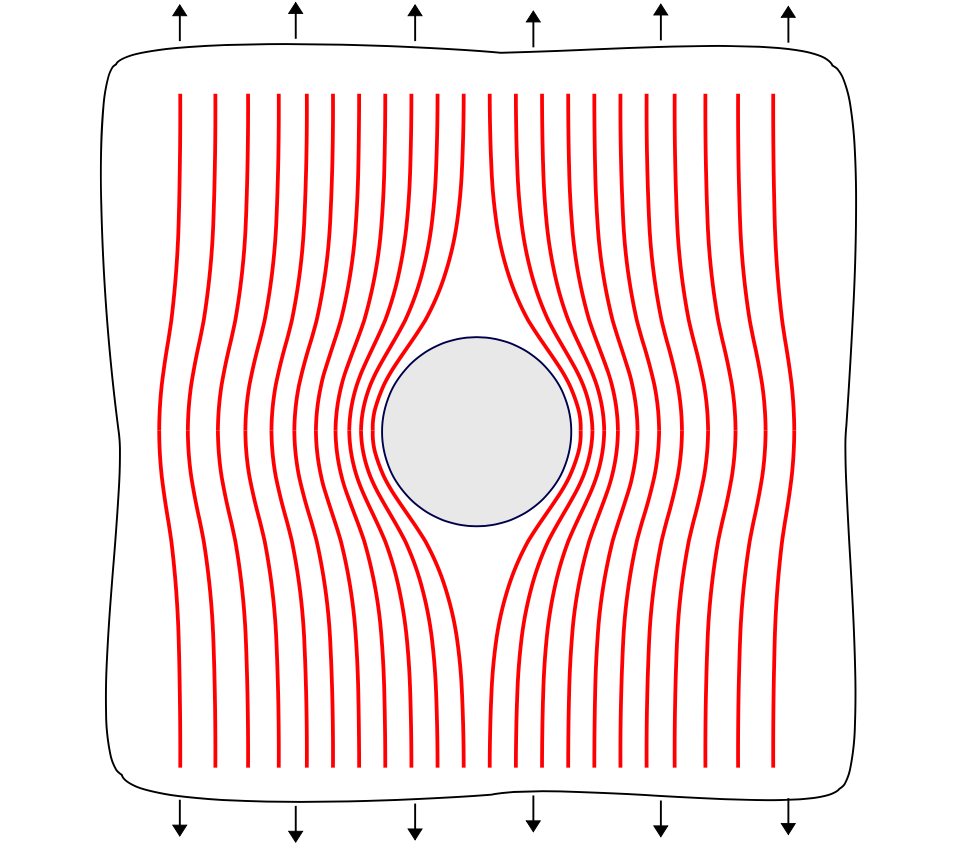
\includegraphics[scale=0.15]{Stress.png}
  	\end{center}
  \caption{Example of stress concentration}
\end{figure}
\linebreak\par
This study shall focus on the stress concentration analysis of aluminium plates featuring a single circular cutout. The location of the cutout with respect to the plate shall be varied, whilst the length and height of the plate are also varied.

%--------------------------------------------------------------------------------------------------------------------------------------------------------------------------------------------------------------------------
% THEORY
%--------------------------------------------------------------------------------------------------------------------------------------------------------------------------------------------------------------------------
\section{Theory} % Section title
Hooke's law predicts that there will be a linear relationship between the force, $F$, applied to a plate and the displacement, $u$, which it undergoes,
\begin{equation} % Equation 1. Hooke's Law
	F = ku
\end{equation}
where $k$ is the "stiffness" of the plate. Equation (1) applies  to a plate so long as it is made of a material that displays linear behaviour within  the range of applied forces. When conducting experiments it is far more useful to work in terms of stress, $\sigma$, and strain, $\varepsilon$. So equation (1) may be manipulated by the use of the cross sectional area of the plate, $A$, and its length, $L$.
\begin{equation} % Equation 2. Dividing through by A and multiplying top & bottom by L.
	\frac{F}{A} = \frac{kL}{A}\frac{u}{L}
\end{equation}
Given that $\sigma = \frac{F}{A}$, $\varepsilon = \frac{u}{L}$ and $E = \frac{kL}{A}$, where $E$ is the Young's modulus of the material, this my be re-wrote as,
\begin{equation} % Equation 3. Stress = Youngs modulus/Strain
	\sigma = E \varepsilon
\end{equation}
If a discontinuity were to be introduced in to a thin plate \cite{plates} there will be a localised increase in stress, known as a stress concentration, around the discontinuity. Imagine a thin rectangular plate containing a circular cutout, where the plate is much larger than the cutout. As stress is $Force/area$ and the area of the plate at the point of the cutout has undergone a reduction there will be a localised increase in the stress state around the cutout. Consider the case displayed in \textit{Figure 2} below, 
% Figure 2. Example of a fractured plate.
\begin{figure}[!ht]
	\centering
		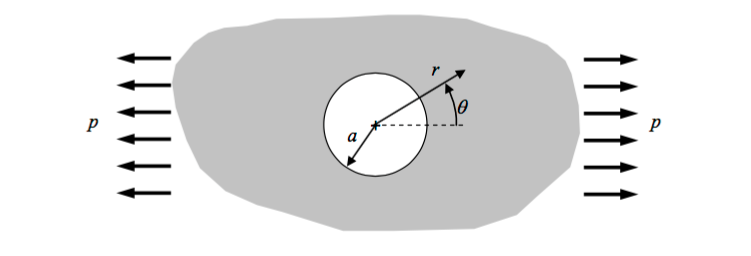
\includegraphics[width=0.5\textwidth]{Fracture.png}
	\caption{Fracture in a thin plate}
\end{figure}
\linebreak
where, $p$, is the uniaxial far-field loading, $a$, is the radius of the circular cutout and using a polar co-ordinate system ($r$, $\theta$) as shown. \linebreak Consider the stress state around a circular cutout in an infinite plate subject to uniaxial tension, the stress state at any point ($r$, $\theta$), where $r \geq a$ may be described by the Kirsch equations \cite{Kirch} as shown below, 
\begin{equation} % Equation 4. Radial stress about a fracture.
	\sigma_{rr} = \frac{p}{2}(1-\frac{a^2}{r^2})+\frac{p}{2}(1+\frac{3a^4}{r^4}-\frac{4a^2}{r^2})cos(2\theta)
\end{equation}
\begin{equation} % Equation 5. Hoop stress.
	\sigma_{\theta\theta} = \frac{p}{2}(1+\frac{a^2}{r^2})-\frac{p}{2}(1+\frac{3a^4}{r^4})cos(2\theta)
\end{equation}
\begin{equation} % Equation 6. Shear stress.
	\tau_{r\theta} = -\frac{p}{2}(1-\frac{3a^4}{r^4}+\frac{2a^2}{r^2})sin(2\theta)
\end{equation}
When $r = a$ this reduces to.
\begin{equation} % Equation 7. r = a, case for radial stress.
	\sigma_{rr} = \tau_{r\theta} = 0
\end{equation}
\begin{equation} % Equation 8. r = a, case for hoop stress.
	\sigma_{\theta\theta} = p(1-2cos(2\theta)
\end{equation}
The radial stress, $\theta_{rr}$, and shear stress, $\tau_{r\theta}$, equal zero at the cutout as it is a free surface. However, the hoop stress, $\sigma_{\theta\theta}$, 
has a value $-p \leq \sigma_{\theta\theta} \leq 3p$ as shown in equation (8). The maximum value of stress occurs when $\theta = \pm\frac{\pi}{2}$ and the minimum occurs when $\theta = 0$ or $\pi$. As the plate is described as being thin, it may be assumed that all the stress fields are confined to the x-y plane meaning that the plate is acting under plane  stress \cite{planestress}. Therefore the following relationships are valid,
\begin{equation} % Equation 9.  Plane strain implications
	\varepsilon_{rr} = \frac{1}{E}(\sigma_{rr}-\nu\sigma_{\theta\theta})
\end{equation}
\begin{equation} % Equation 10. Plane strain implications
	\varepsilon_{\theta\theta} = \frac{1}{E}(\sigma_{\theta\theta}-\nu\sigma_{rr})
\end{equation}
\begin{equation} % Equation 11. Plane strain implications
	\gamma_{r\theta} = \frac{\tau_{r\theta}}{G}
\end{equation}
\begin{equation} % Equation 12. Shear modulus
	G = \frac{E}{2(1 + \nu)}
\end{equation}
where $E$ is Young's modulus, $\nu$ is Poisson's ratio and $G$ is the shear modulus of the material. 
\linebreak\par 
The stress state around the circular cutout is often quoted in terms of a stress concentration factor, $K_{t}$ (equation (13)), which is the ratio of the maximum stress around a feature (in this example the circular cutout) to the stress which would've been present at that ($r, \theta$) co-ordinate had the feature not been there, this is known as the far-field stress or  nominal stress, $\sigma_{nom}$. 
\begin{equation} % Equation 13. Stress concentration ratio.
	K_{t} = \frac{\sigma_{max}}{\sigma_{nom}}
\end{equation}
Therefore  a circular cutout in an infinite plate has a stress concentration factor $K_{t}$ = 3 (see equation (8)). However this is only valid for cutouts which are small in comparison to the plate. There exists no analytical solution for how the stress concentration factor changes as the cutout stops being small with respect to the plate. Instead design charts may be consulted, experiments may be performed or computational simulations may be carried out to provide a value of $K_{t}$ for the plate dimensions in question. 

%--------------------------------------------------------------------------------------------------------------------------------------------------------------------------------------------------------------------------
% EXPERIMENTAL METHOD	
%--------------------------------------------------------------------------------------------------------------------------------------------------------------------------------------------------------------------------
\section{Experimental Method}
\subsection{Experimental procedure}
A thin plate of aluminium with one end fixed such that it could undergo no horizontal displacement and the other end loaded to a desired force via the loading rig, was assembled  as can be seen in \textit{Figure 3}
% Figure 3 Apparatus.
\begin{figure}[!ht]
	\centering
		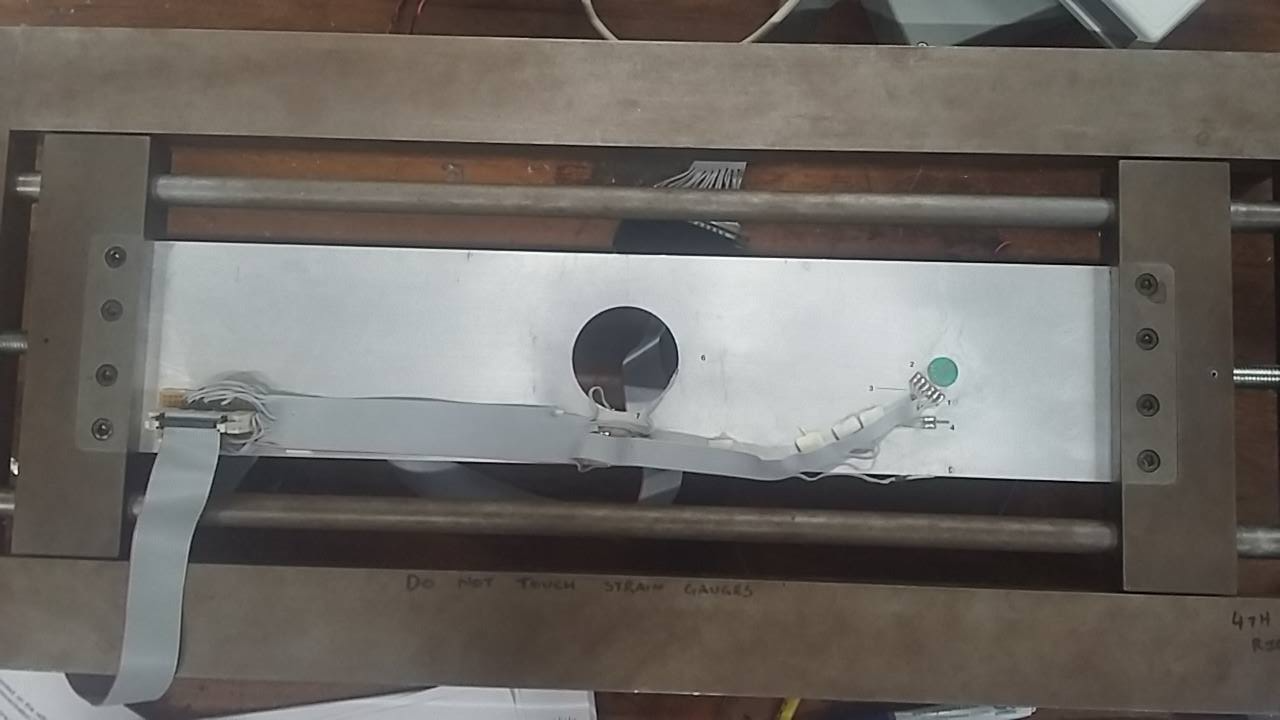
\includegraphics[width=0.5\textwidth]{Apperatus.png}
	\caption{The setup used for this experiment}
\end{figure} 
Nine strain gauge meters were then placed on the surface aluminium plate. Of which two were around the perimeter of the circular cutout $\pi$ radians apart. The remaining 7 strain gauges were placed at far-field locations, as may be seen in \textit{Figure 4}. These gauges were attached to a computer and displayed the values of strain recorded. Readings of strain were recorded as opposed to stress as it is far more convenient.
% Figure 4 Gauge positions.
\begin{figure}[!ht]
	\centering
		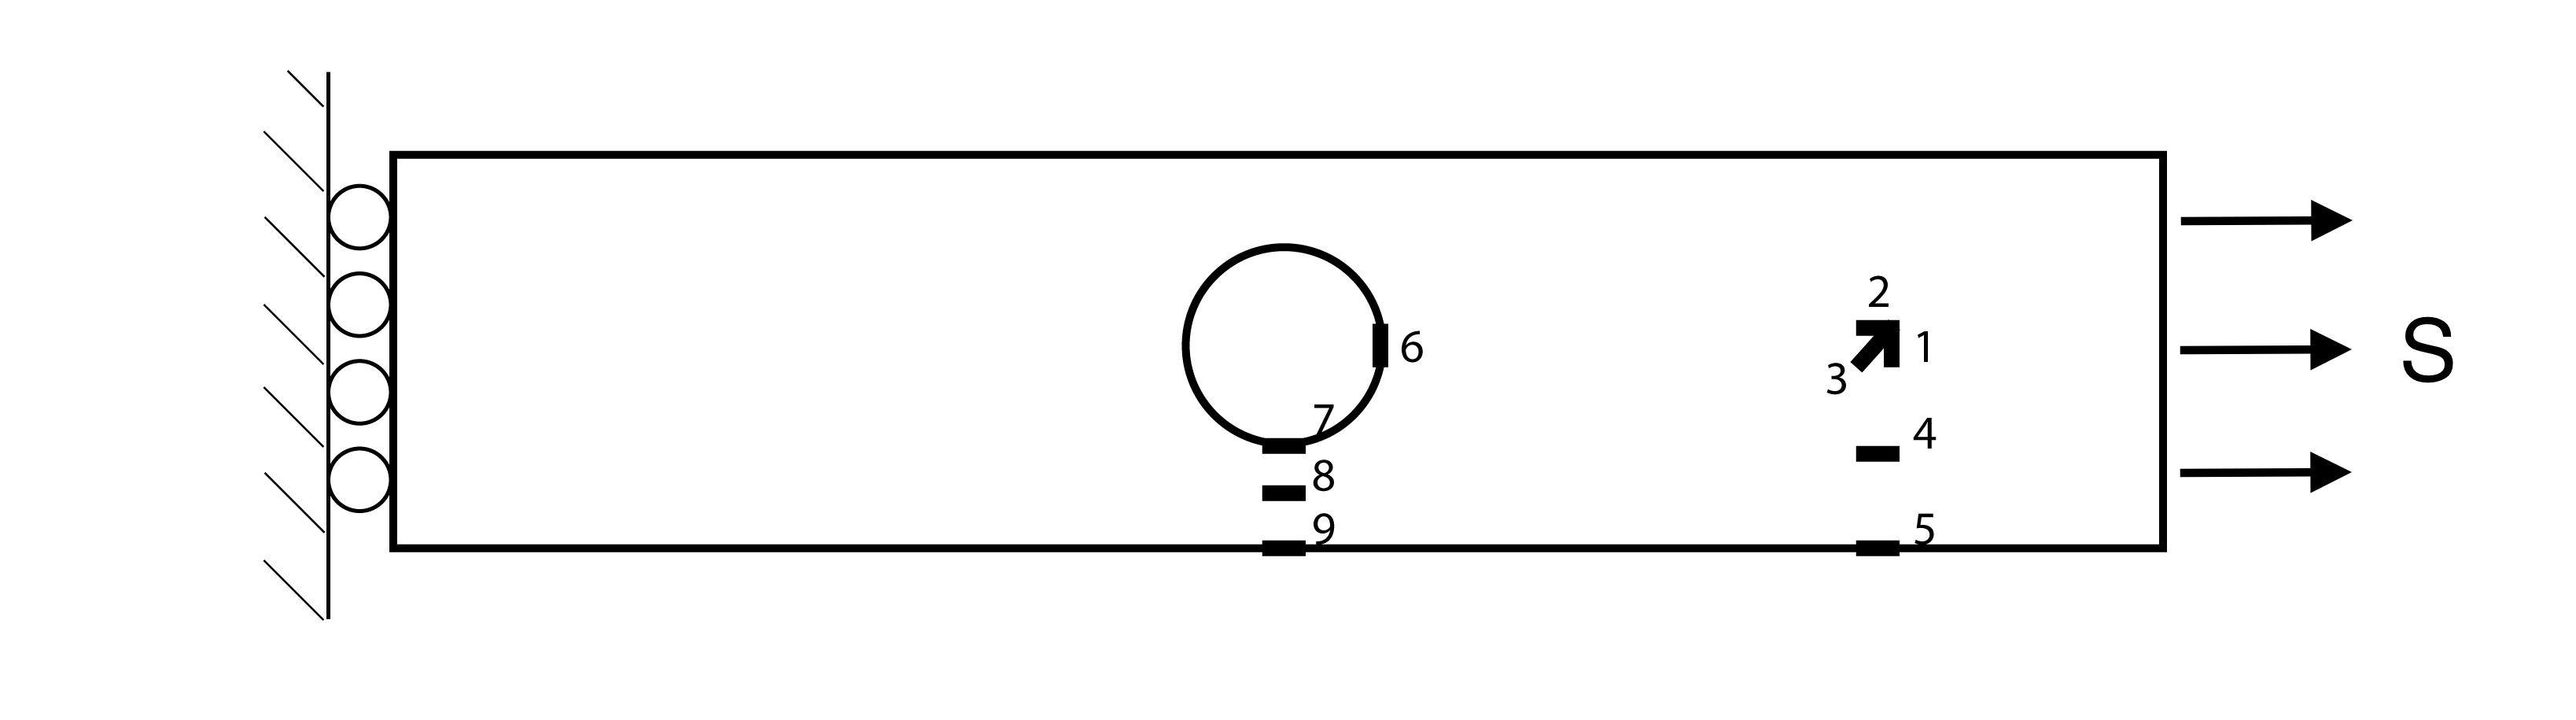
\includegraphics[width=0.5\textwidth]{ComputationalPlate2.png}
	\caption{Strain gauge locations}
\end{figure} 
\par 
Initially the aluminium plate was unloaded so all the strain gauges could be correctly zeroed, then the load was applied until the strain gauge which gave the highest reading was at a strain of $200\mu\varepsilon$, now the values of strain for all nine gauges was noted. The load was then removed and strain gauges zeroed once more. This process was then repeated for loads of $400\mu\varepsilon$, $600\mu\varepsilon$, $800\mu\varepsilon$. The plate was not to be loaded past $1000\mu\varepsilon$. This whole process was repeated three times to reduce the possibility of any outlier results skewing data.

\subsection{Computational Simulation}
The second stage to this investigation was to use the \textit{Concept Analyst} software to analyse a plate as shown below in $Figure  5$ For the analysis the plate length was varied from L = H to L = 10H, taking new readings every H. For every value of $L$, readings were taken for different values of the ratio of $a/c$ and $e/c$ as shown in \textit{Figure 5} below.
% Figure 5. Computational analysis plate.
\begin{figure}[!ht]
\centering
\includegraphics[height=4cm,width=0.5\textwidth]{ComputationalPlate.png}
\caption{Computational analysis plate.}
\end{figure} 

%--------------------------------------------------------------------------------------------------------------------------------------------------------------------------------------------------------------------------
% RESULTS AND DISCUSSION 
%--------------------------------------------------------------------------------------------------------------------------------------------------------------------------------------------------------------------------
\section{Results and Discussion}

\subsection{Experimental data analysis}

\subsubsection{Determining a value for $K_{t}$ for the aluminium plate featuring a circular cutout} 

The graph below (\textit{Figure 6}) displays the average reading for each of the 4 applied loads for gauge 2 plotted on the x-axis against the average readings for gauge 7 plotted on the y-axis. The reason that gauge 2 was plotted on the x-axis was due to its physical location, it could be considered far-field from the feature on the plate and therefore the stress state at that location would be the nominal stress, $\sigma_{nom}$, so it may be treated as a reference gauge. Gauge 7 was plotted on the y-axis due to it being at the feature and would therefore represent the maximum stress state on the plate, $\sigma_{max}$. 
% Figure 6. Gauge 2 readings plotted against gauge 7 readings
\begin{figure}[!ht]
	\centering
		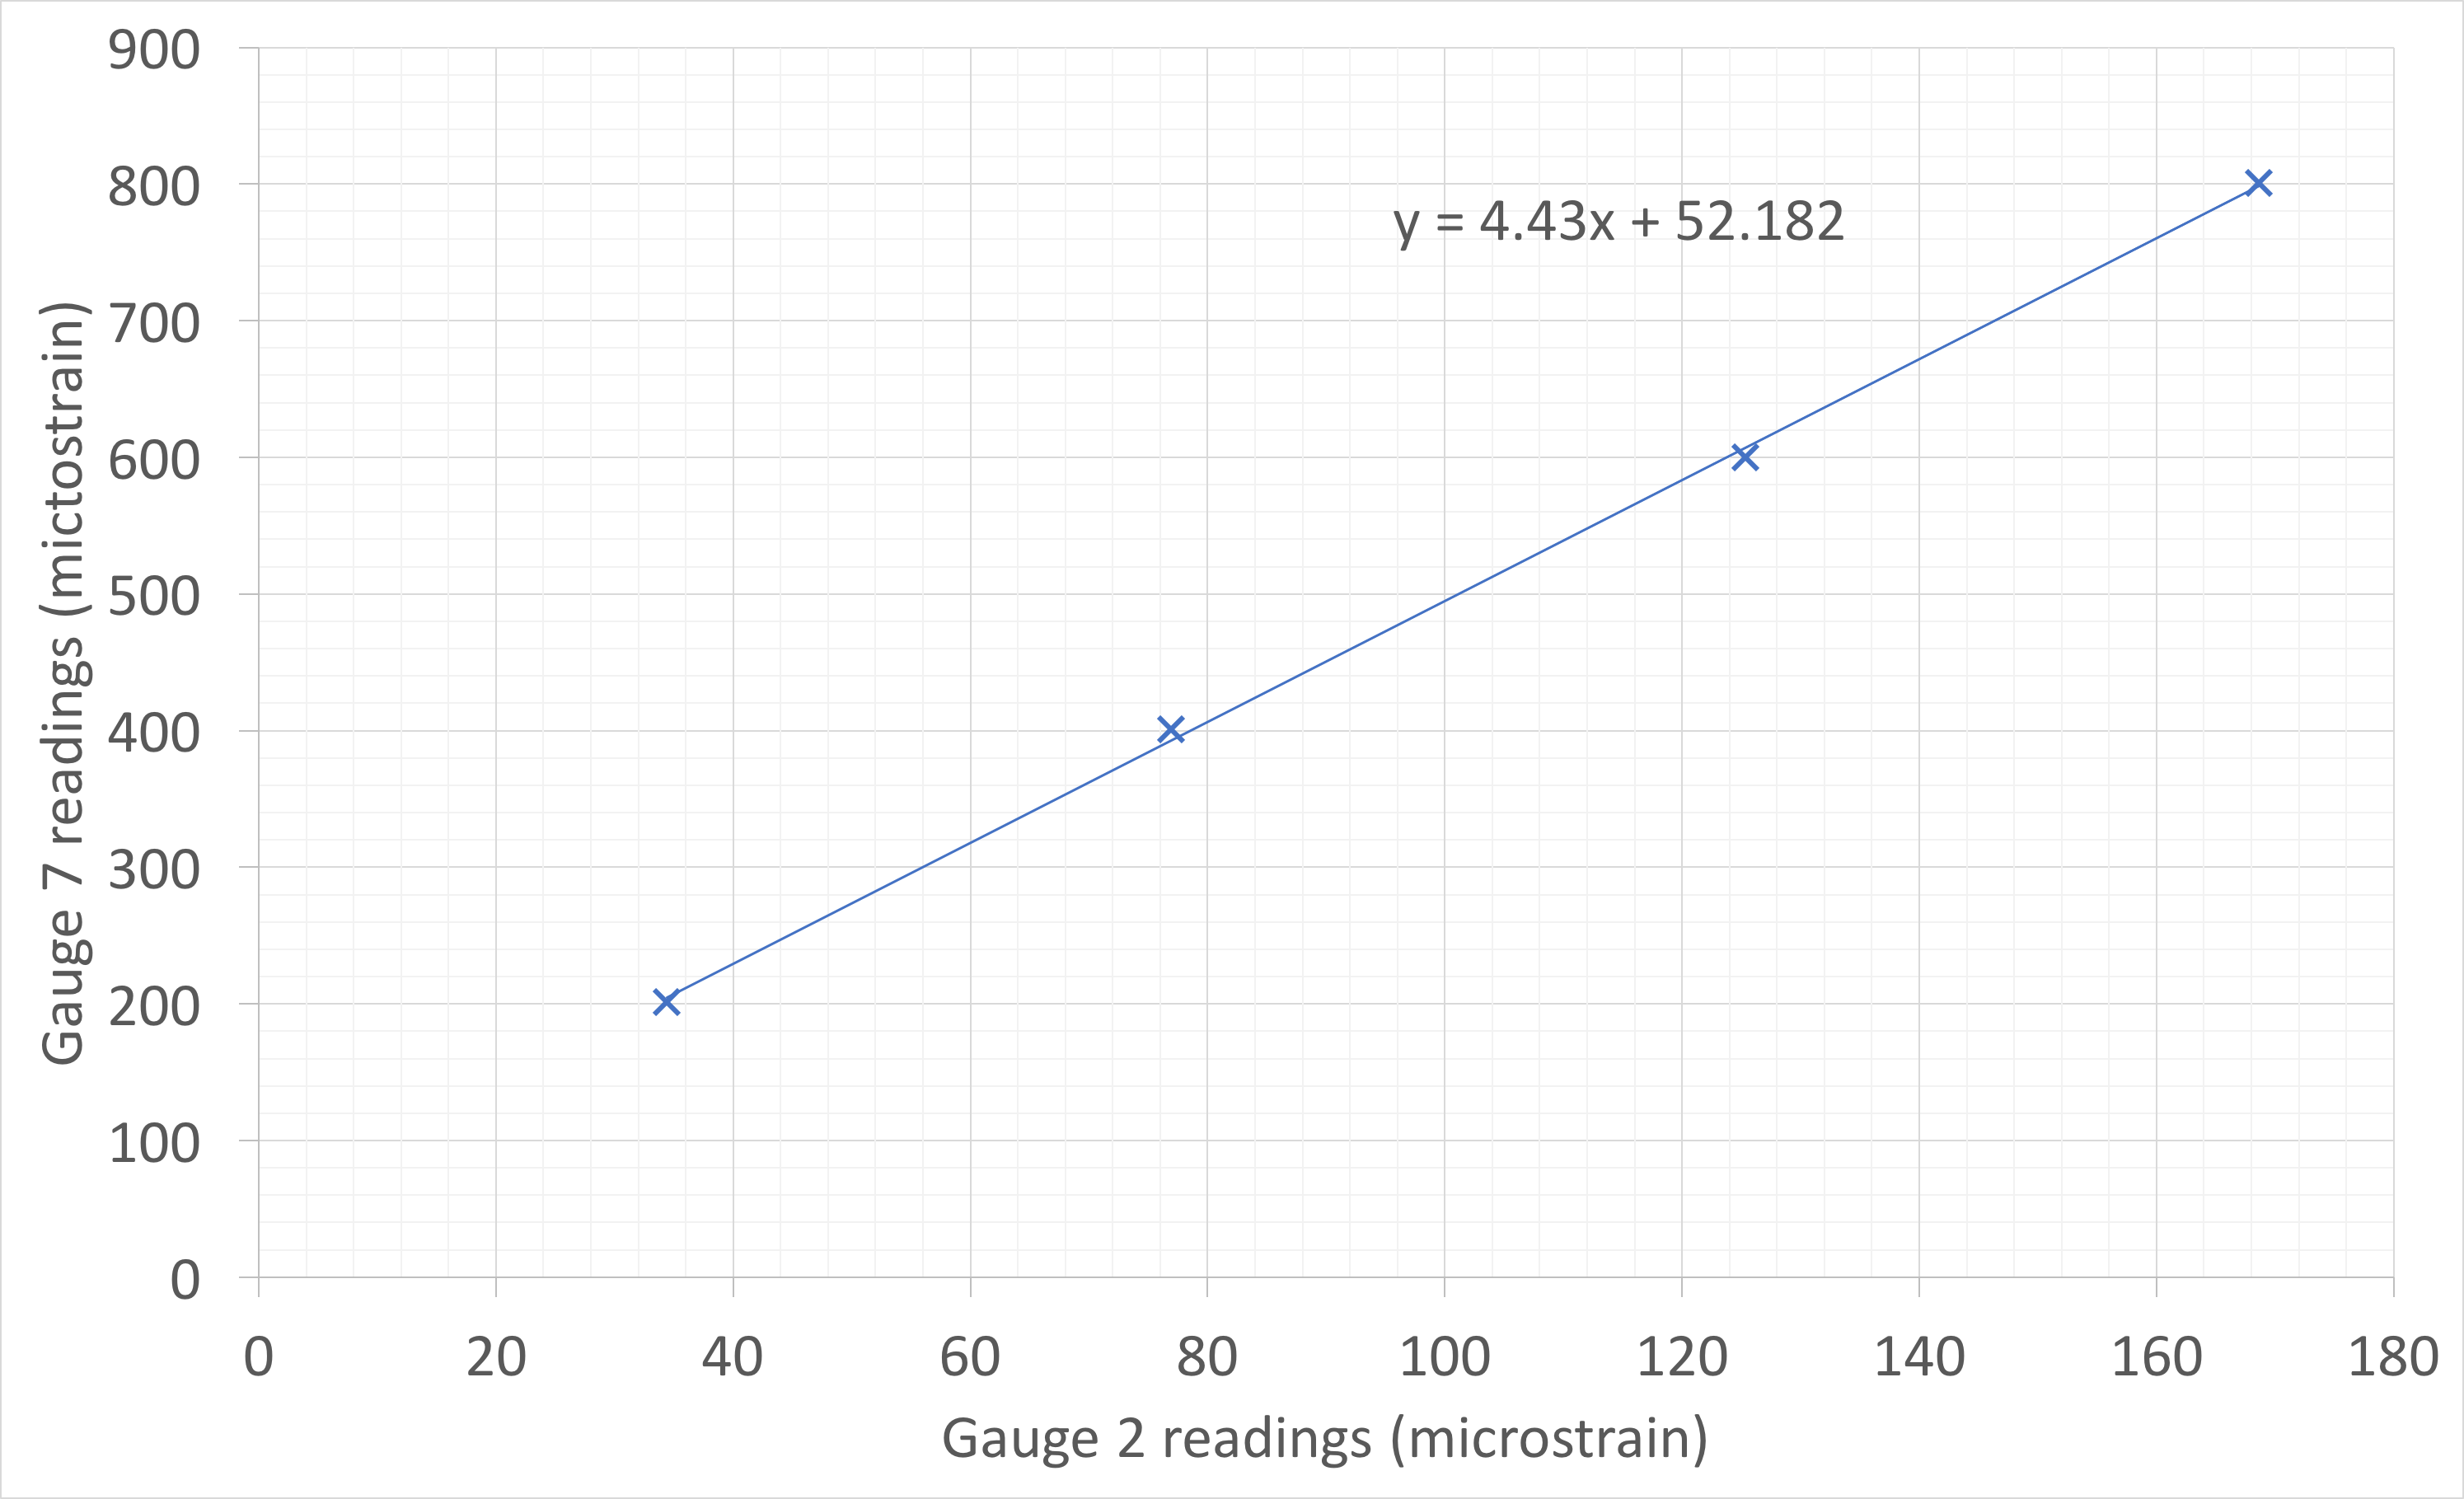
\includegraphics[width=0.5\textwidth]{G2G7.png}
	\caption{Gauge 2 readings plotted against gauge 7 readings}
\end{figure} 
The gradient of the line plotted on \textit{Figure 6} is therefore the $K_{t}$ value for this circular cutout on this plate. (see \textit{equation 13}). The gradient of the line and therefore value of $k_{t}$ is determined to be 4.43. Meaning that the point of maximum stress about the cutout for a plate of these dimensions  will be 4.43 times larger than the far-field stress. This is something that would have to be under consideration should the plate be used in a system where it would be under load, as this may lead to the stress around the cutout to be larger than the yield stress, $\sigma_{y}$, of the material. 
\par 
Upon performing a computational simulation on a plate made of aluminium of the same dimensions in \textit{Concept Analyst} produces a value of $K_{t}$ which is 4.31, meaning that there is a difference of 0.09 between the theoretical value and the experimentally acquired value which in terms of percentage difference is 2.08\%.
\par  
Uncertainties in the experimental values obtained which may account for the difference in the experimentally obtained and the computational simulation obtained results from this experiment may have arose from the zeroing of the strain gauges. The values displayed never settled exactly on zero, but instead fluctuated approximately within the range $-0.03\geq 0 \geq 0.03$. In addition to this, when measuring the plate dimensions for the computational simulation the only equipment available to hand was a standard ruler with a sensitivity of $\pm0.5mm$, meaning that measurements made were limited in how accurate they could be. So when these values were input into the concept analysis software the uncertainty will effect the value of $K_{t}$ obtained from the simulation. A further source of this error may have come from a strain gauge being damaged whilst handling the plate. These gauges are very delicate pieces of equipment so can easily be damaged. Any such damage could result in the readings from the gauge being inaccurate. 

\subsubsection{Determining Poisson's ratio for the aluminium plate}

A plate which is loaded under tension will become narrower in its cross-section. So the positive axial strain, $\varepsilon_{xx}$, produced by applying a tensile force produces an accompanying transverse strain, $\varepsilon_{yy}$. How large the strains are is governed by the value of the Poisson's ratio, $\nu$, which is defined as,
\begin{equation} % Equation 14. Poissons ratio
\nu = -\frac{\delta\varepsilon_{yy}}{\delta\varepsilon_{xx}} 
\end{equation}
Gauge 1 is placed in a far-field location perpendicular to gauge 2, which is used as the reference gauge. Therefore gauge 1 may be considered as, $\varepsilon_{yy}$, while gauge 2 is considered as, $\varepsilon_{xx}$.
 The value for, $\nu$, can therefore be determined by calculating the gradient of the line for gauge 1. From \textit{Figure 7} it is determined that $\nu = 0.32$ which is comparable to the value the actual value for Poisson's ratio for an aluminium alloy which is ~0.32 \cite{Aluminium}.  
% Figure 7. Graph used to determine the Poisson's ratio for the aluminium plate
 \begin{figure}[!ht]
	\centering
		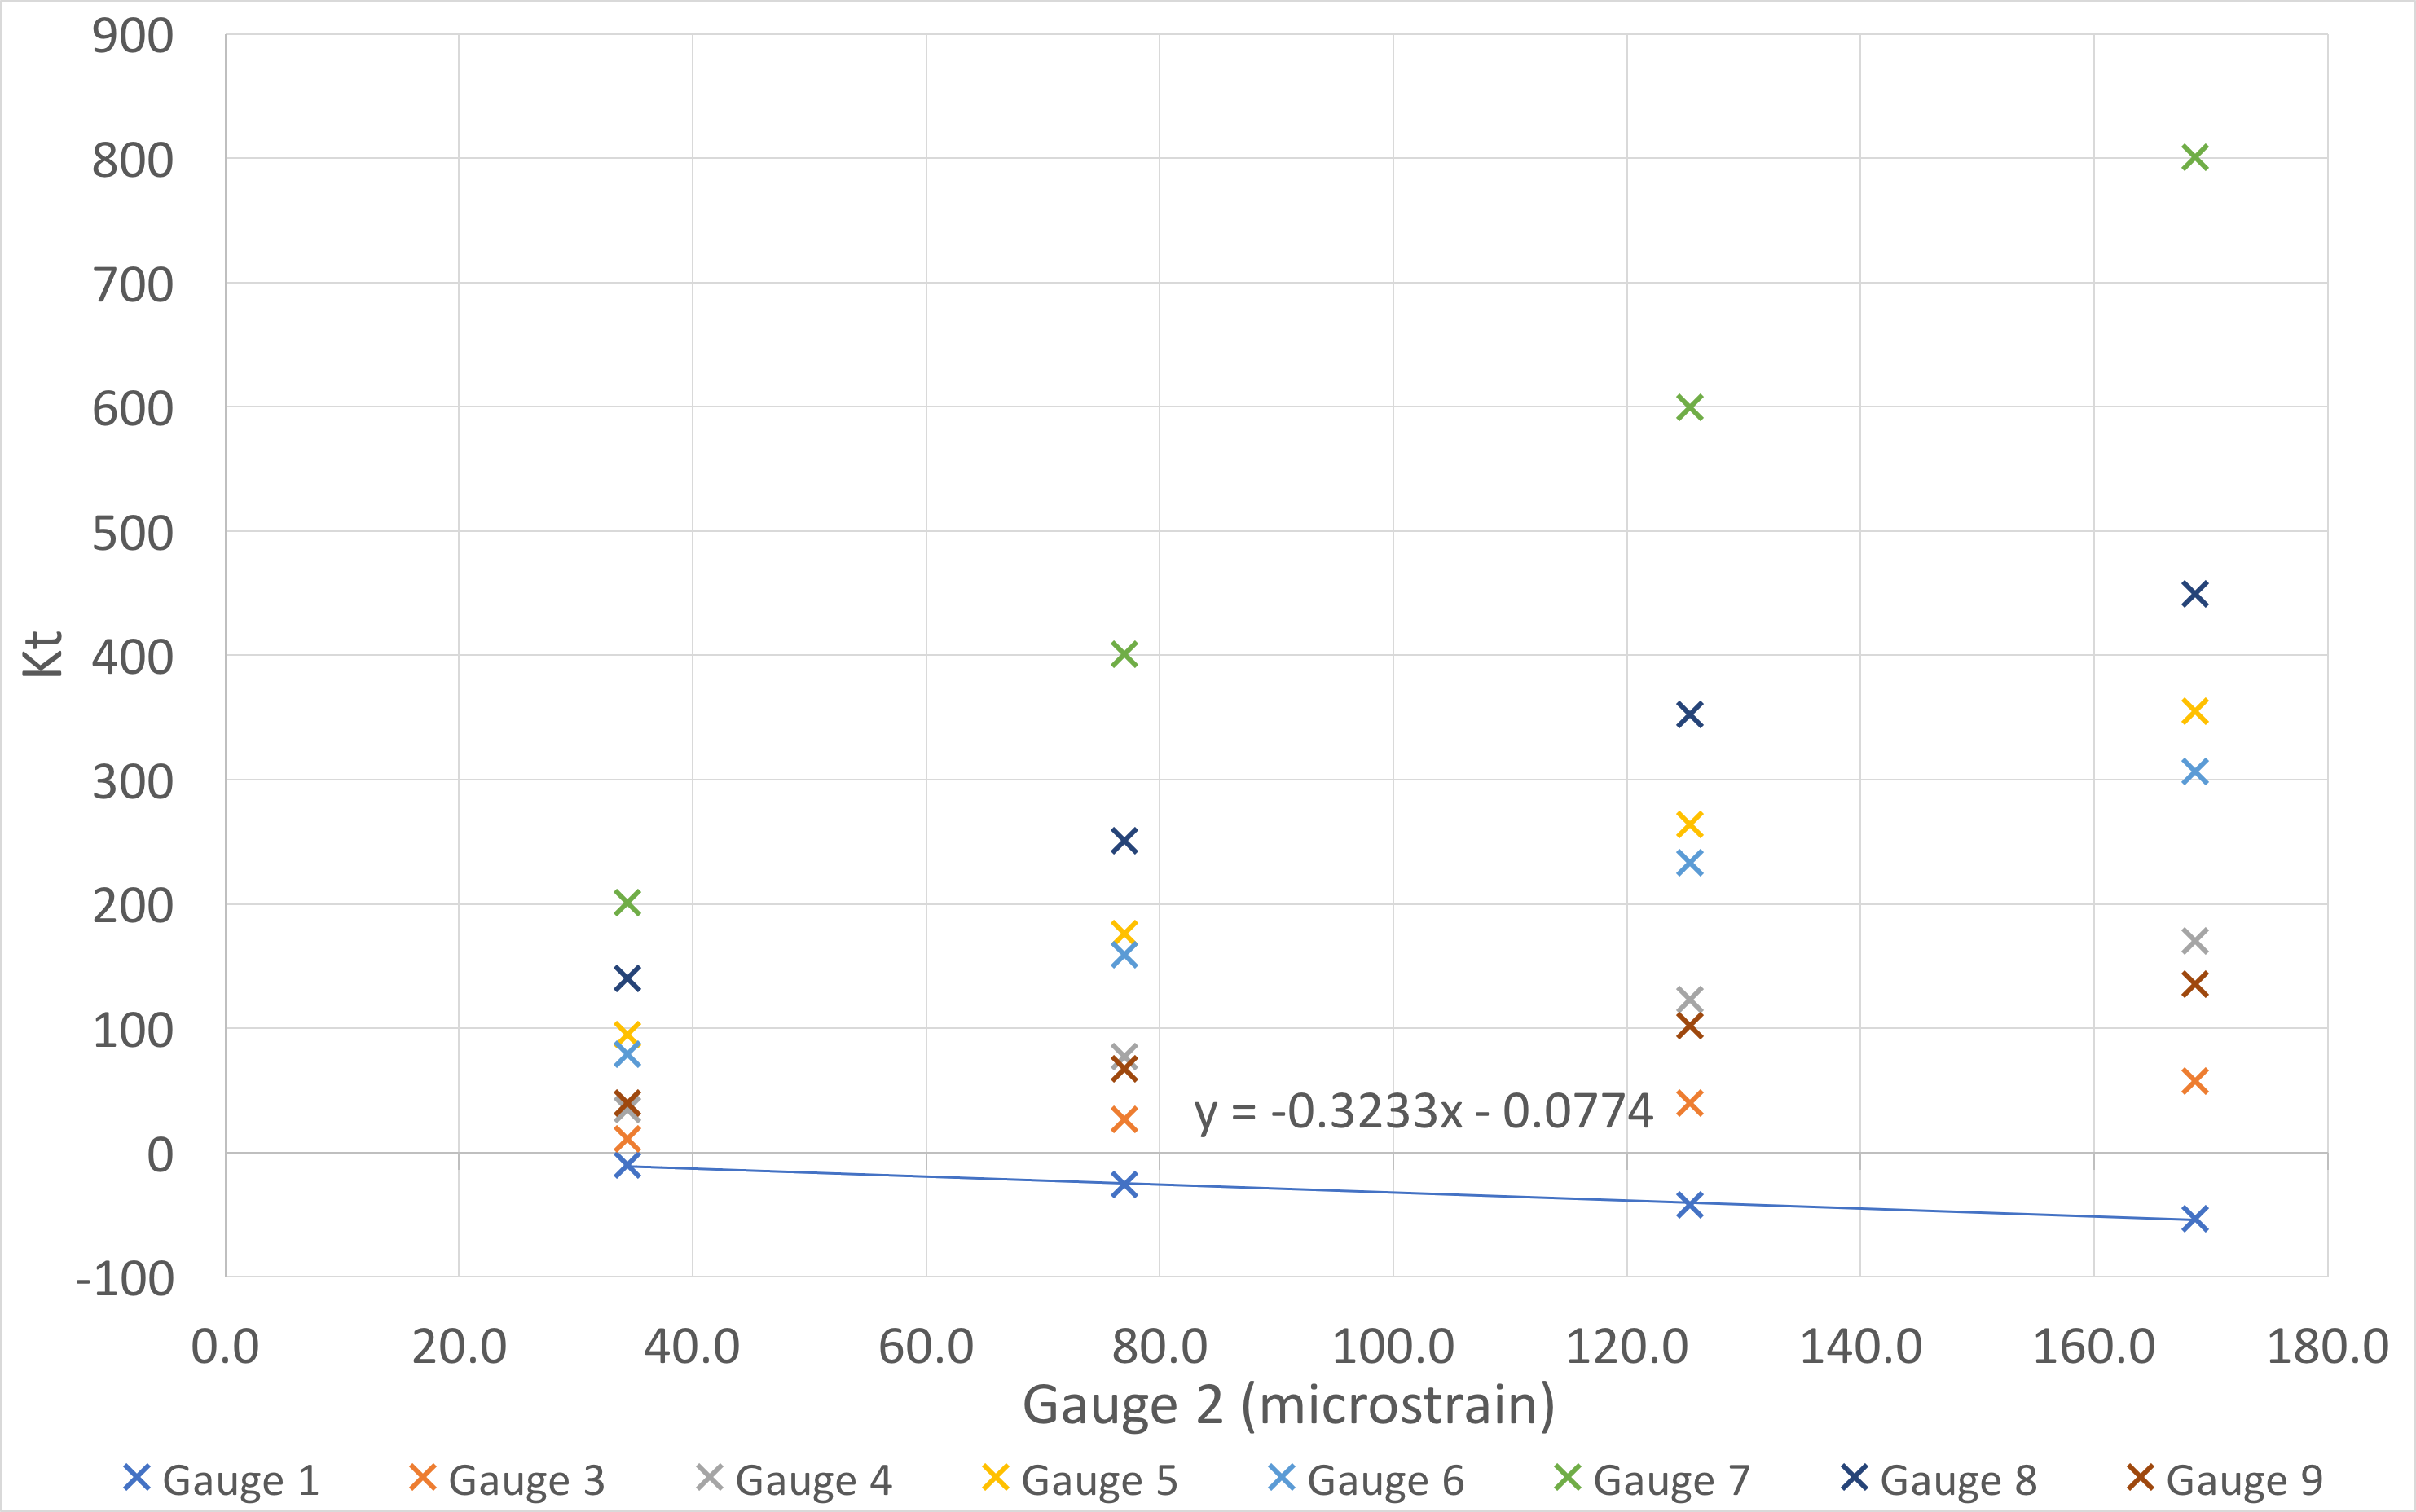
\includegraphics[width=0.5\textwidth]{Poissons.png}
	\caption{Graph used to determine the Poisson's ratio for the aluminium plate}
\end{figure}

\subsection{Computational data analysis}

\subsubsection{How varying a/c  on an infinite plate effects the value of $K_{t}$}

Upon studying \textit{Figure 8} it is apparent that there exists a positive correlation between the value of $K_{t}$ and the value of \textit{a/c}. Meaning that as the size of the cutout increases with respect to the size of the plate, the stress state around the cutout increases. This may be explained by \textit{equations 1} \& \textit{2} which state that the stress within a plate under plane stress is proportional to the amount of force applied. So as the size of the cutout gets larger there is a greater amount of force passing through the gap between the edge of the cutout and the edge of the plate, therefore the localised stress will increase (see $Figure 1$).
% Figure 8. How varying a/c effects the value of Kt 
\begin{figure}[!ht]
	\centering
		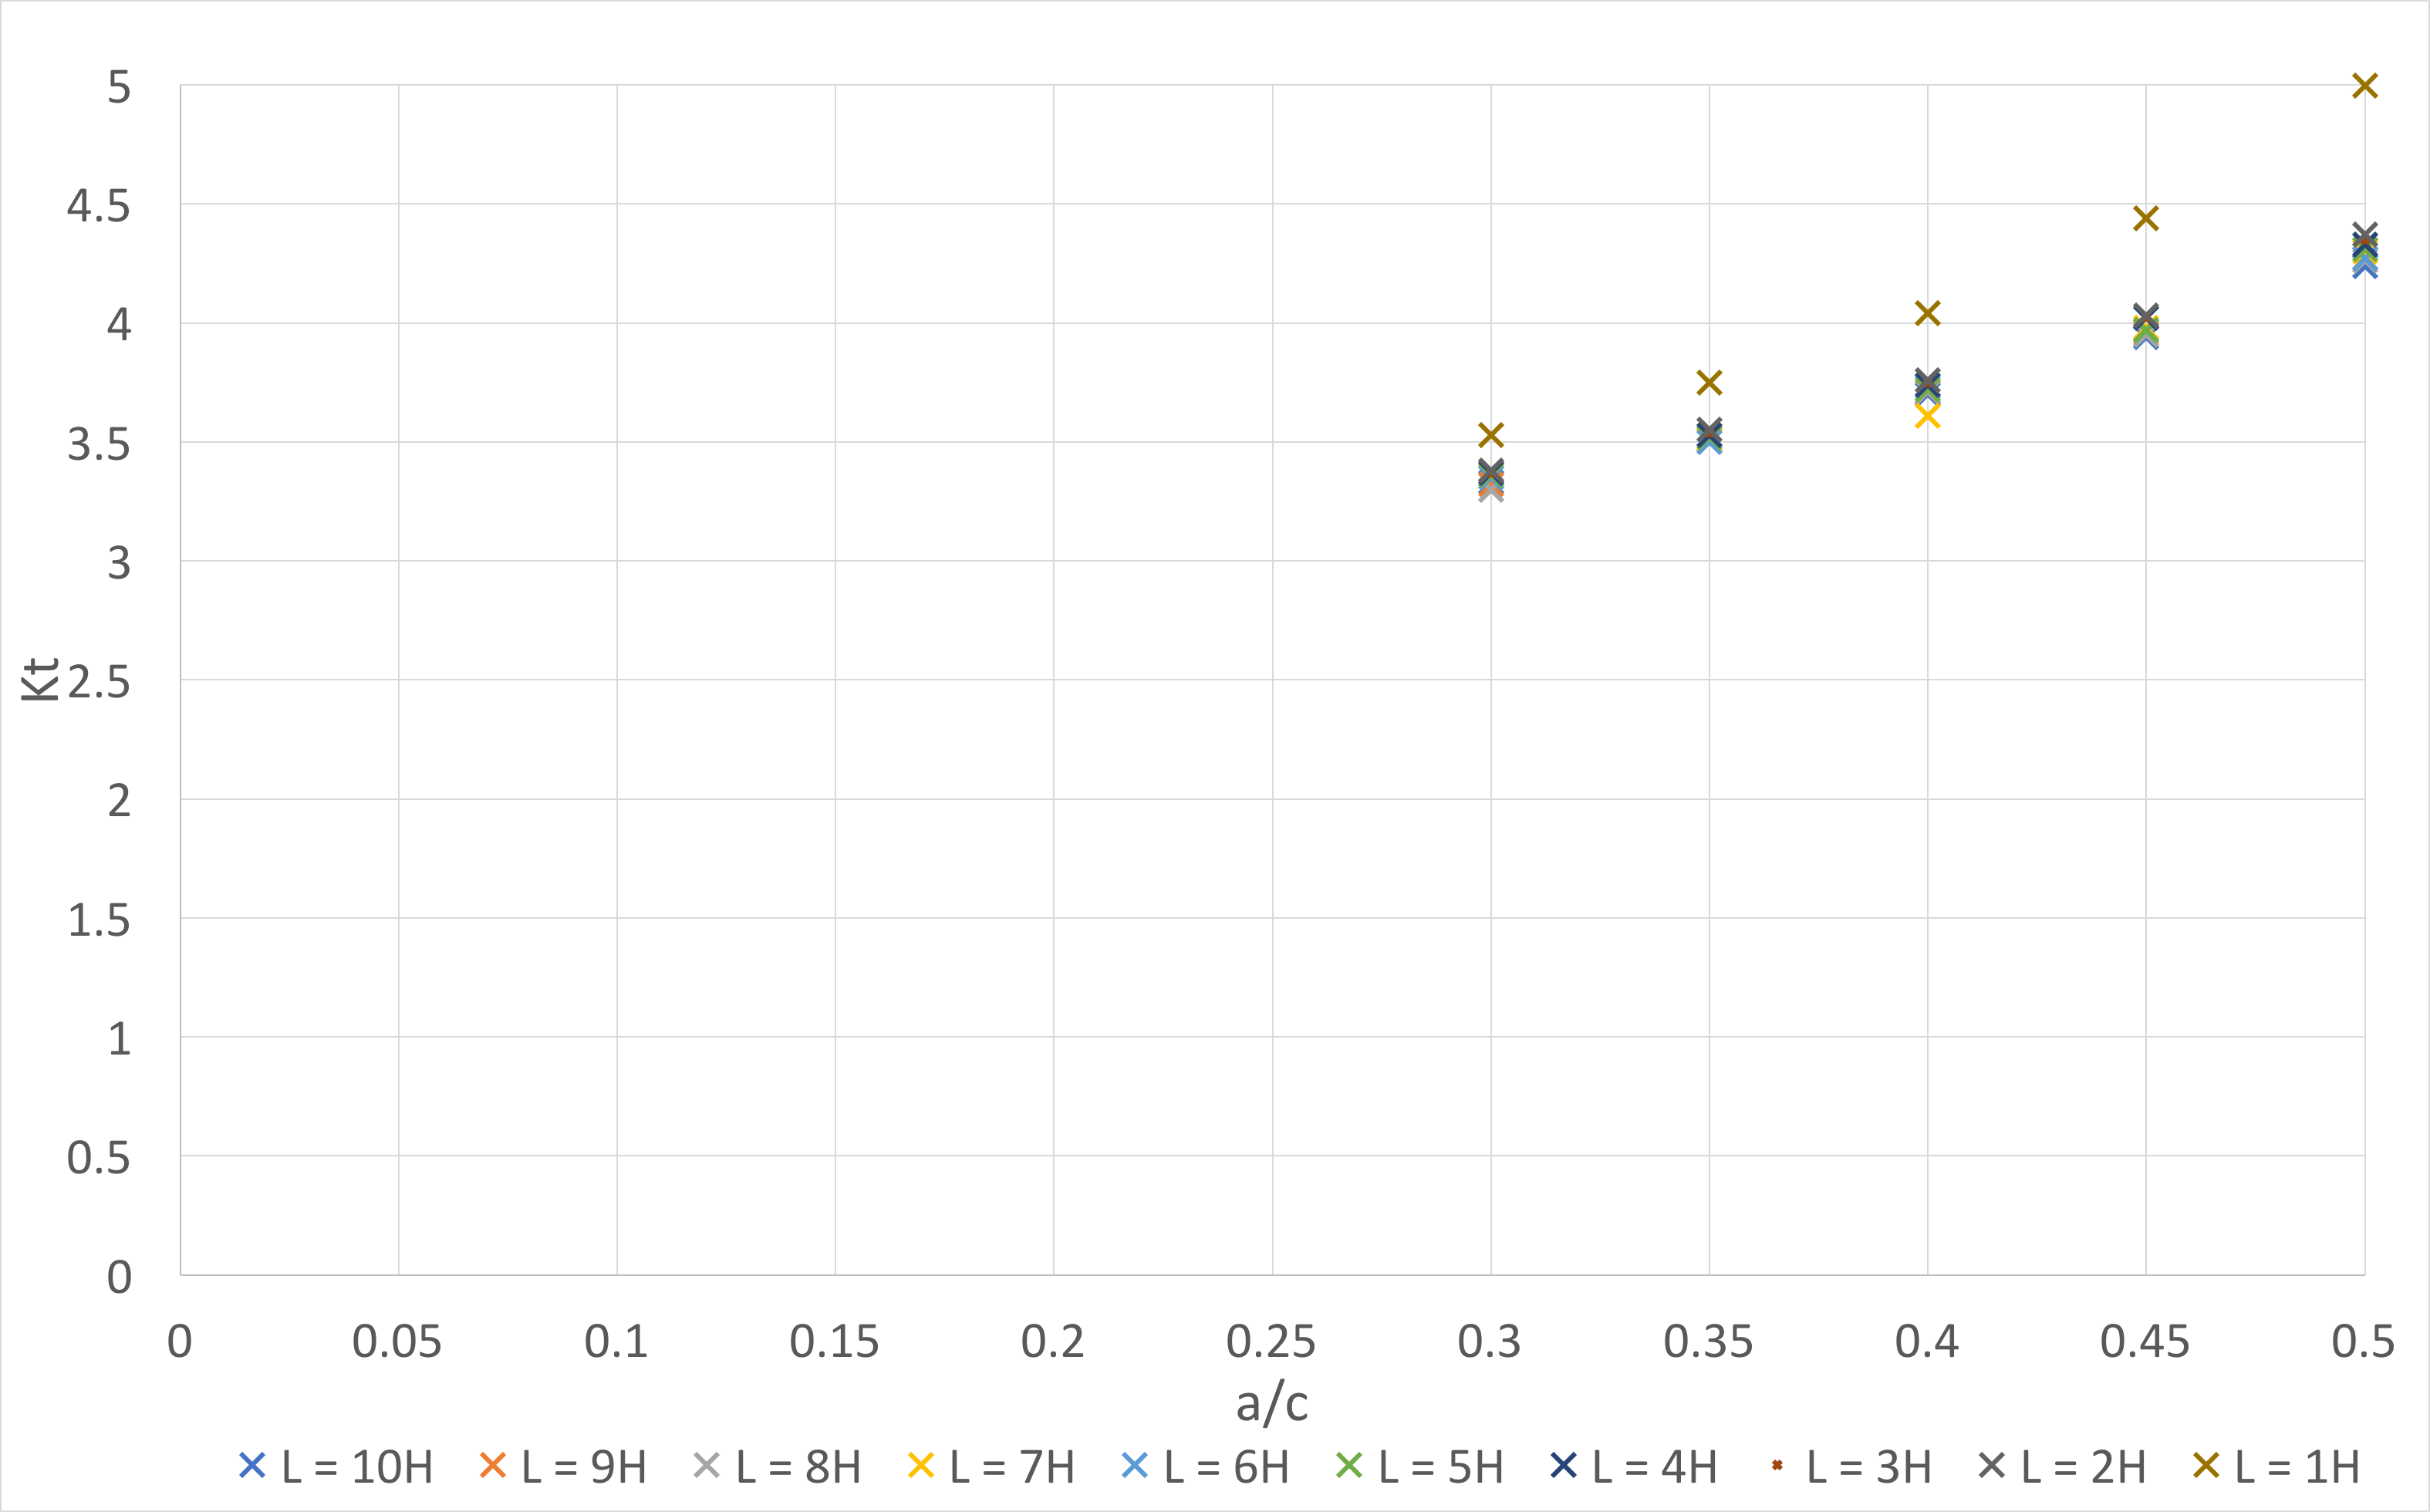
\includegraphics[width=0.5\textwidth]{acKt.png}
	\caption{How varying $a/c$ effects the value of $K_{t}$}
\end{figure}

\subsubsection{How varying e/c on an infinite plate effects the value of $K_{t}$}
Varying the value of $e/c$ effects the fraction of the plate which is between the edge of the cutout and the edge of the plate. Considering \textit{Figure 9} below shows that as e/c is increased, the value of $K_{t}$ decreases. This means that as you decrease the fraction of the plate which is between the edge of the plate and the edge of the cutout, the maximum value of stress in the plate decreases. This may be explained by considering equations 1 \& 2 which state that the stress within a plate under plane stress is proportional to the force applied to the plate. So as the value of $e/c$ is increased, the force per area across the whole plate decreases. As the applied force has not changed, there is now a smaller force acting across the gap between the edge of the cut out and edge of the plate whilst the cross-section of the plate has been increased, therefore there is a smaller maximum stress value. 
 % Figure 9 
\begin{figure}[!ht]
\centering
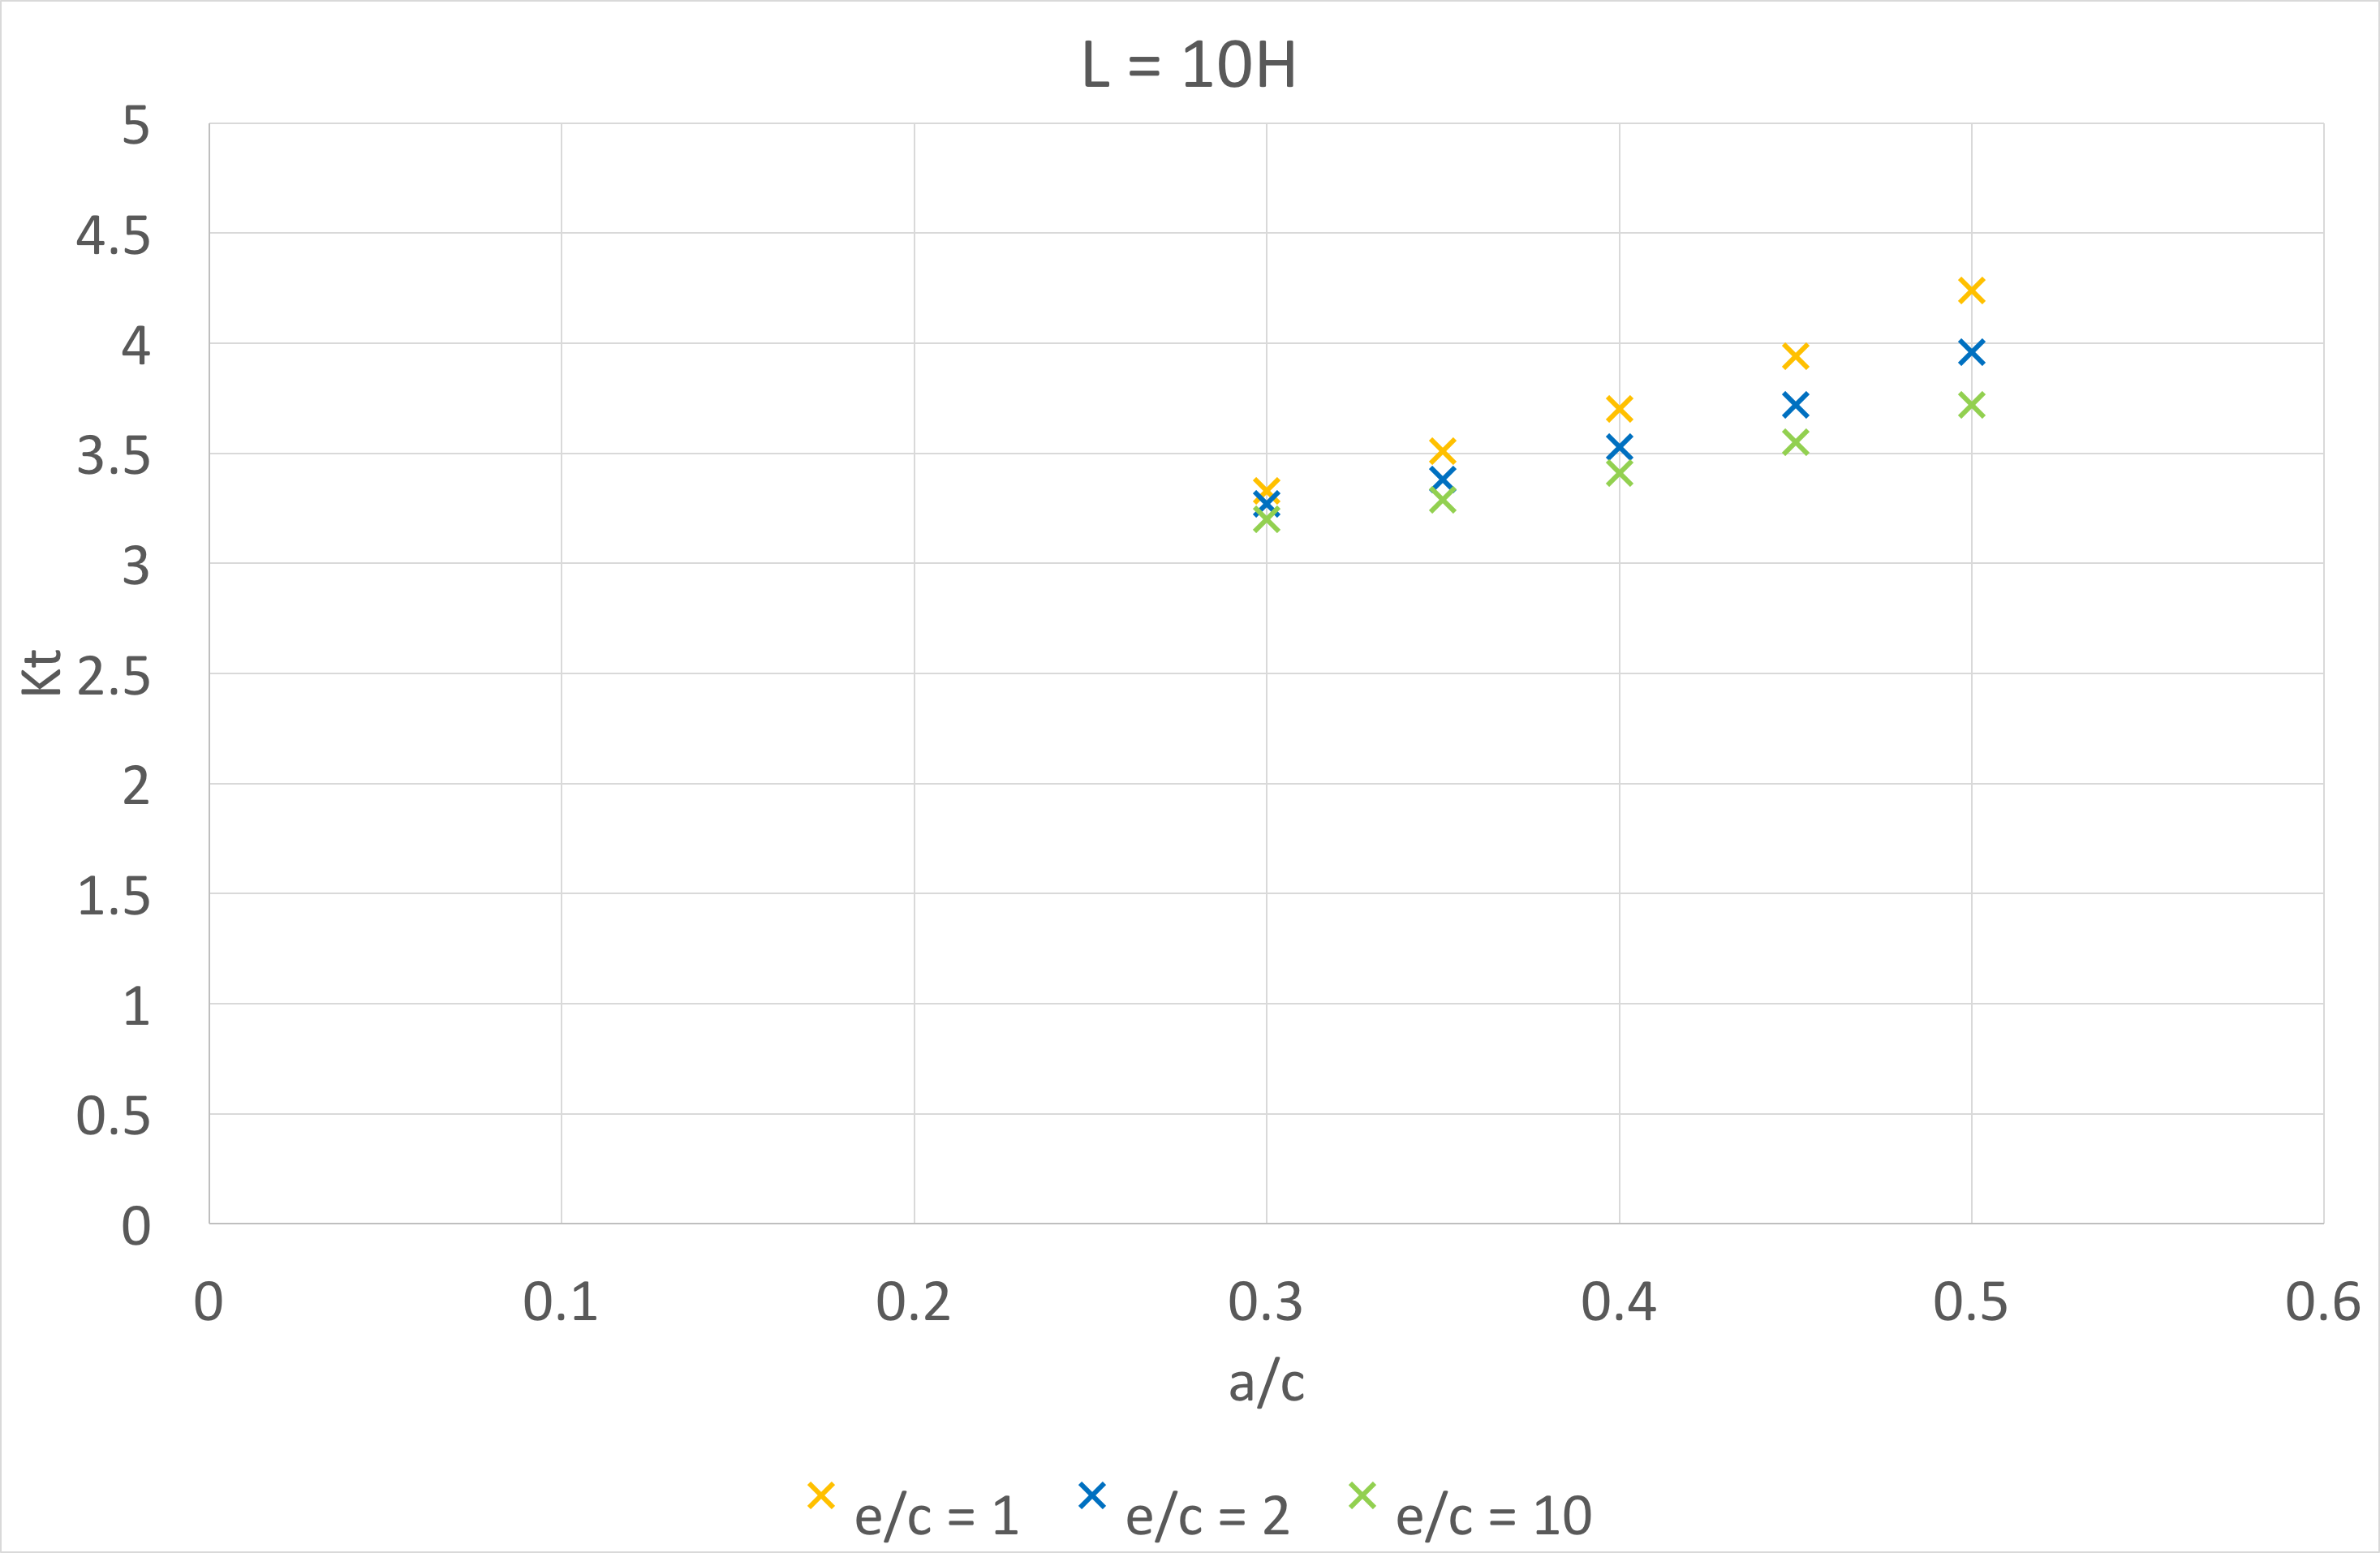
\includegraphics[width=0.5\textwidth]{ec.png}
\caption{How $K_{t}$ varies with e/c}
\end{figure}
 
\subsubsection{How reducing the plates length so it may no longer be assumed to be infinite affects $K_{t}$}

 The experimental data displayed in \textit{Figure 10} below show how the value of $K_{t}$ changes as $L$ is varied. It can be seen that as the plate length is decreased within the range $5H \geq L \geq 10H$, the value of $K_{t}$  remains within a range of $\pm0.1$. Whereas once the plate length drops to $<5H$ there is a clear negative correlation between the plate length and the value of $K_{t}$. Therefore demonstrating that once the plate length drops to below $5H$ it is no longer reasonable to consider the plate as infinite, as any change in the length produces a relatively large increase in the value of $K_{t}$.
 % Figure 10 
\begin{figure}[!ht]
\centering
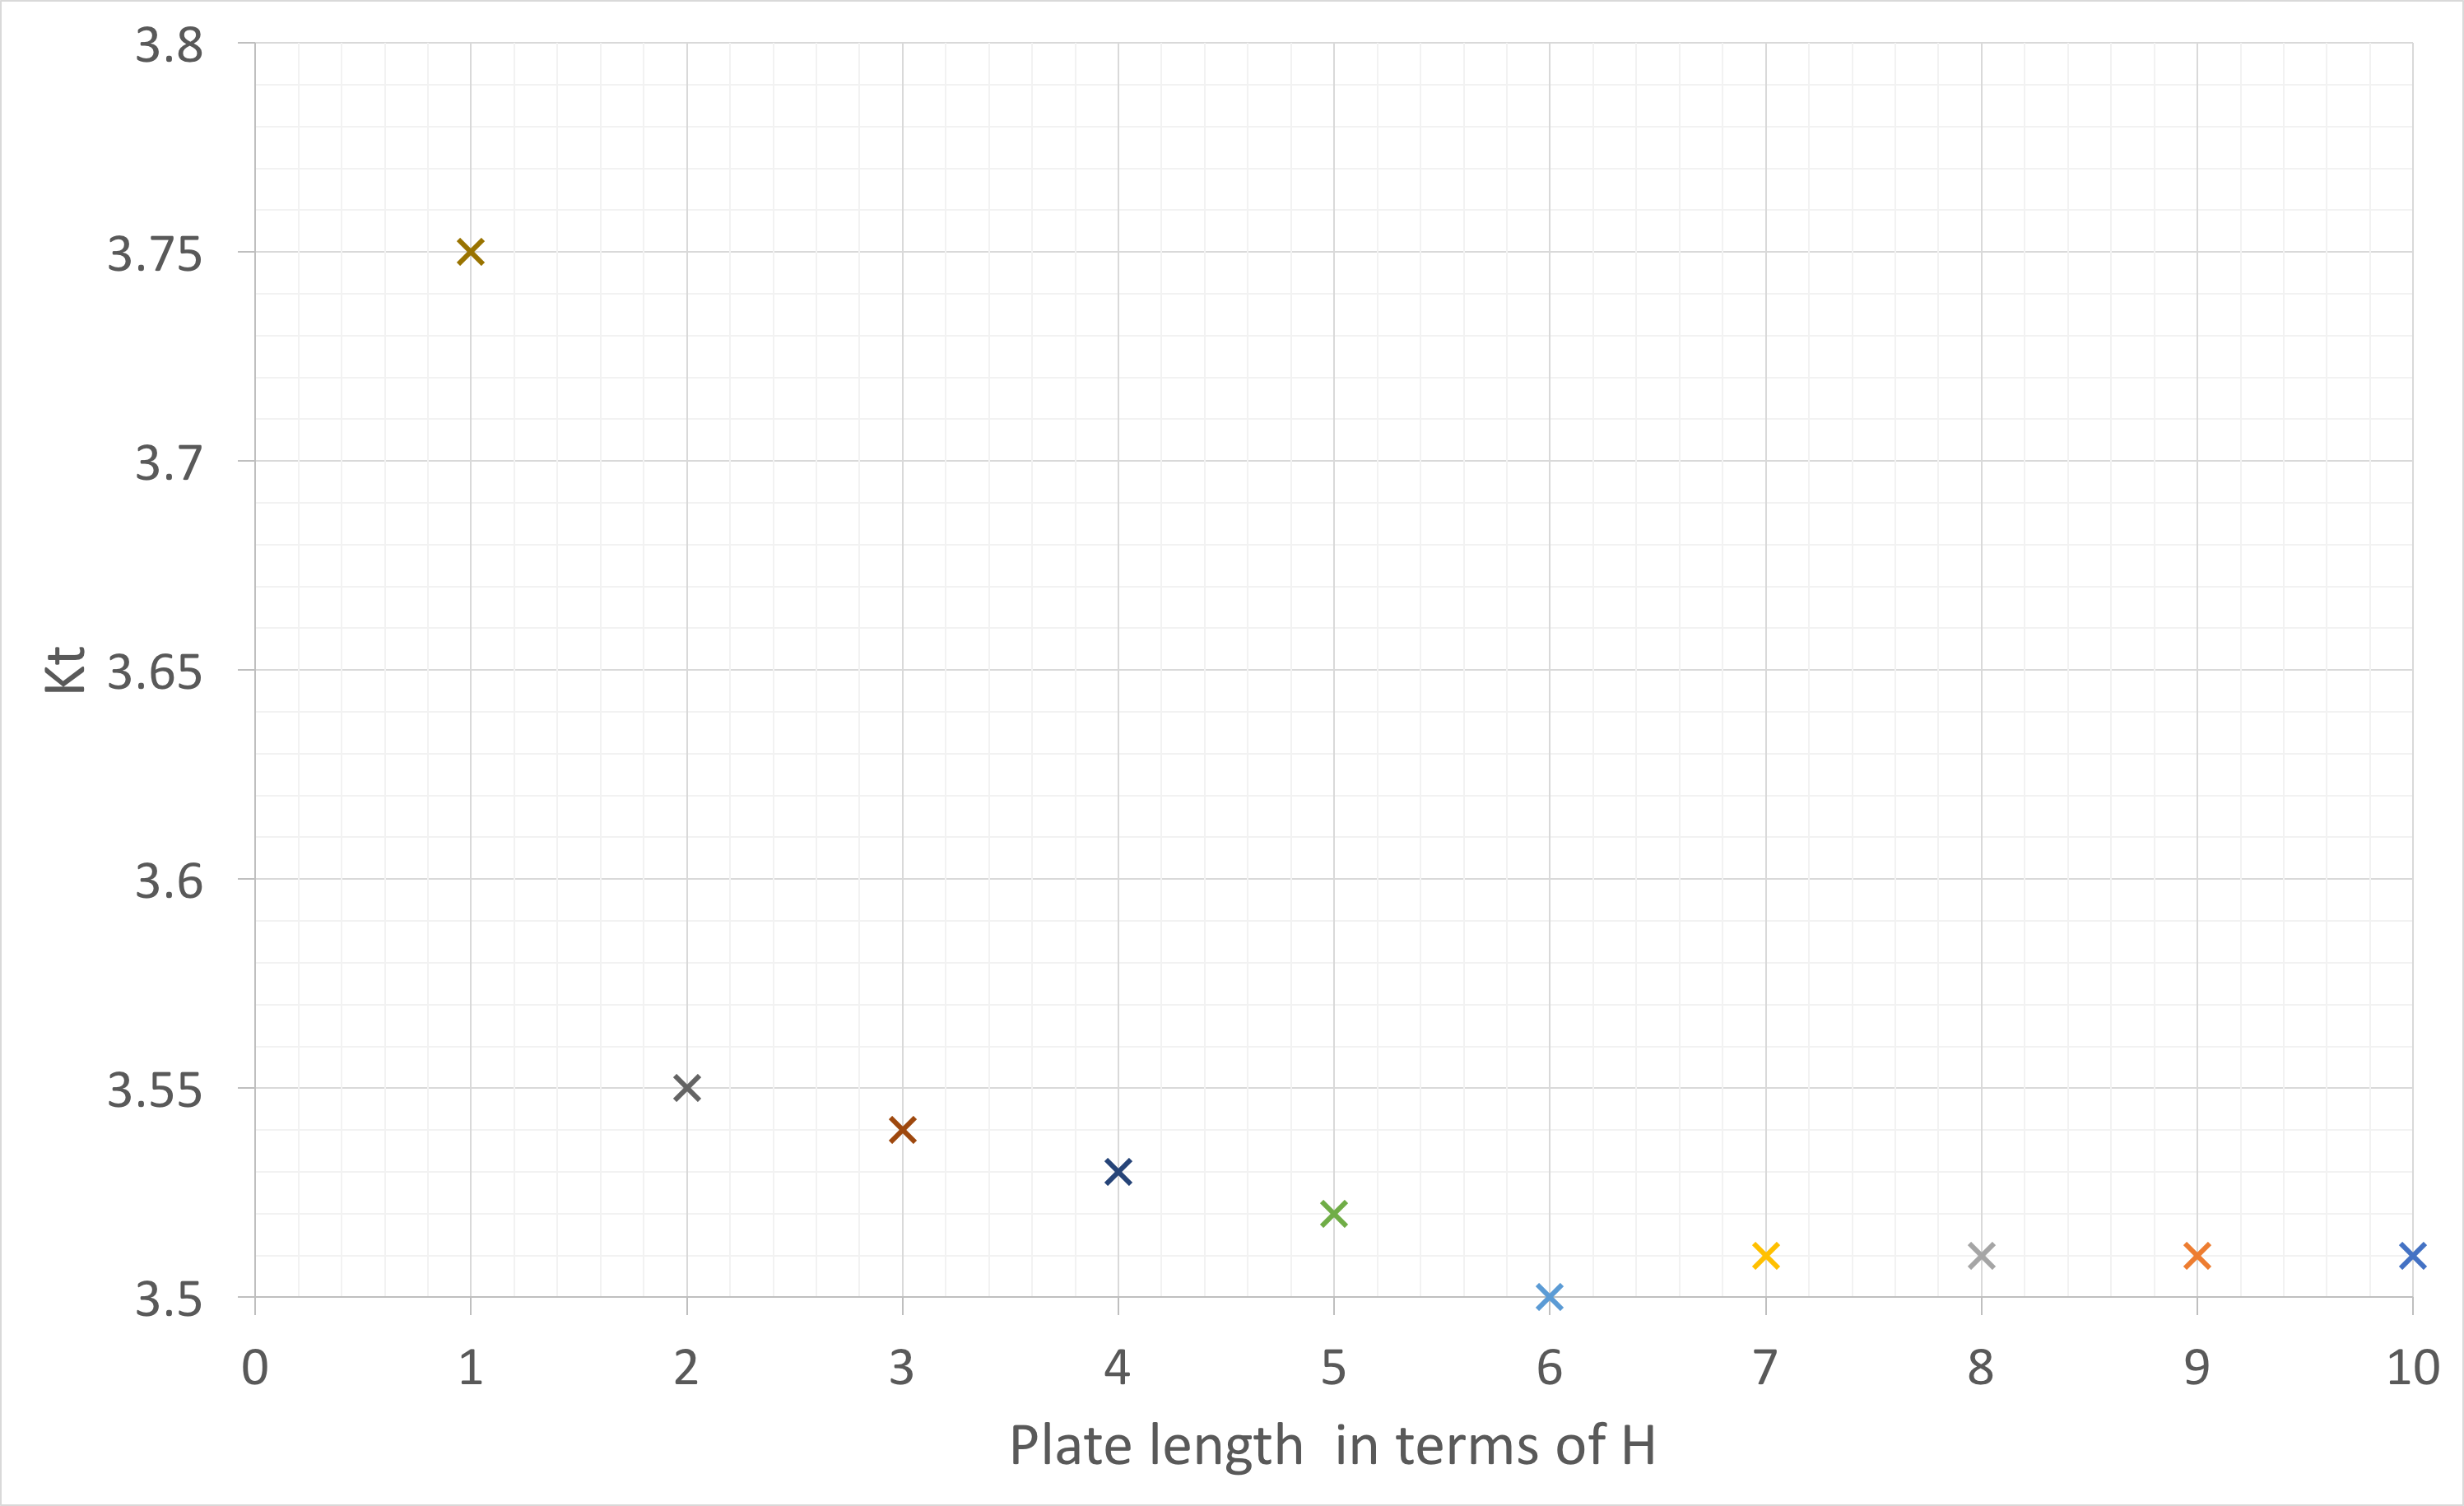
\includegraphics[width=0.5\textwidth]{Lvar.png}
\caption{How $K_{t}$ varies with L}
\end{figure}
\linebreak\linebreak\linebreak\linebreak
\\ \par
\textit{Figures 11} \& \textit{12} provide a more detailed look into how the value of $K_{t}$ varies as the length of the plate reduces to a value whereby it no longer represents an infinite plate. From studying the \textit{Figures 11} \& \textit{12} there appears to be very little difference in the values of $K_{t}$ as the plate length decreases. With the minimum value of $K_{t}$ for $L=5H$ being $3.2$ and the minimum value of $K_{t}$ for $L=4H$ being $3.2$. When the maximum value of $K_{t}$ is considered for these two cases. The respective values are $K_{t}=4.31$ for when $L=5H$, and $K_{t}=4.33$ for when $L=4H$, producing a percentage difference of $\%0.46$, so whilst considering the infinite and non-infinite plate there is very little difference in the stress concentration factor. 
 % Figure 11 & 12
\begin{figure}[!ht]
    	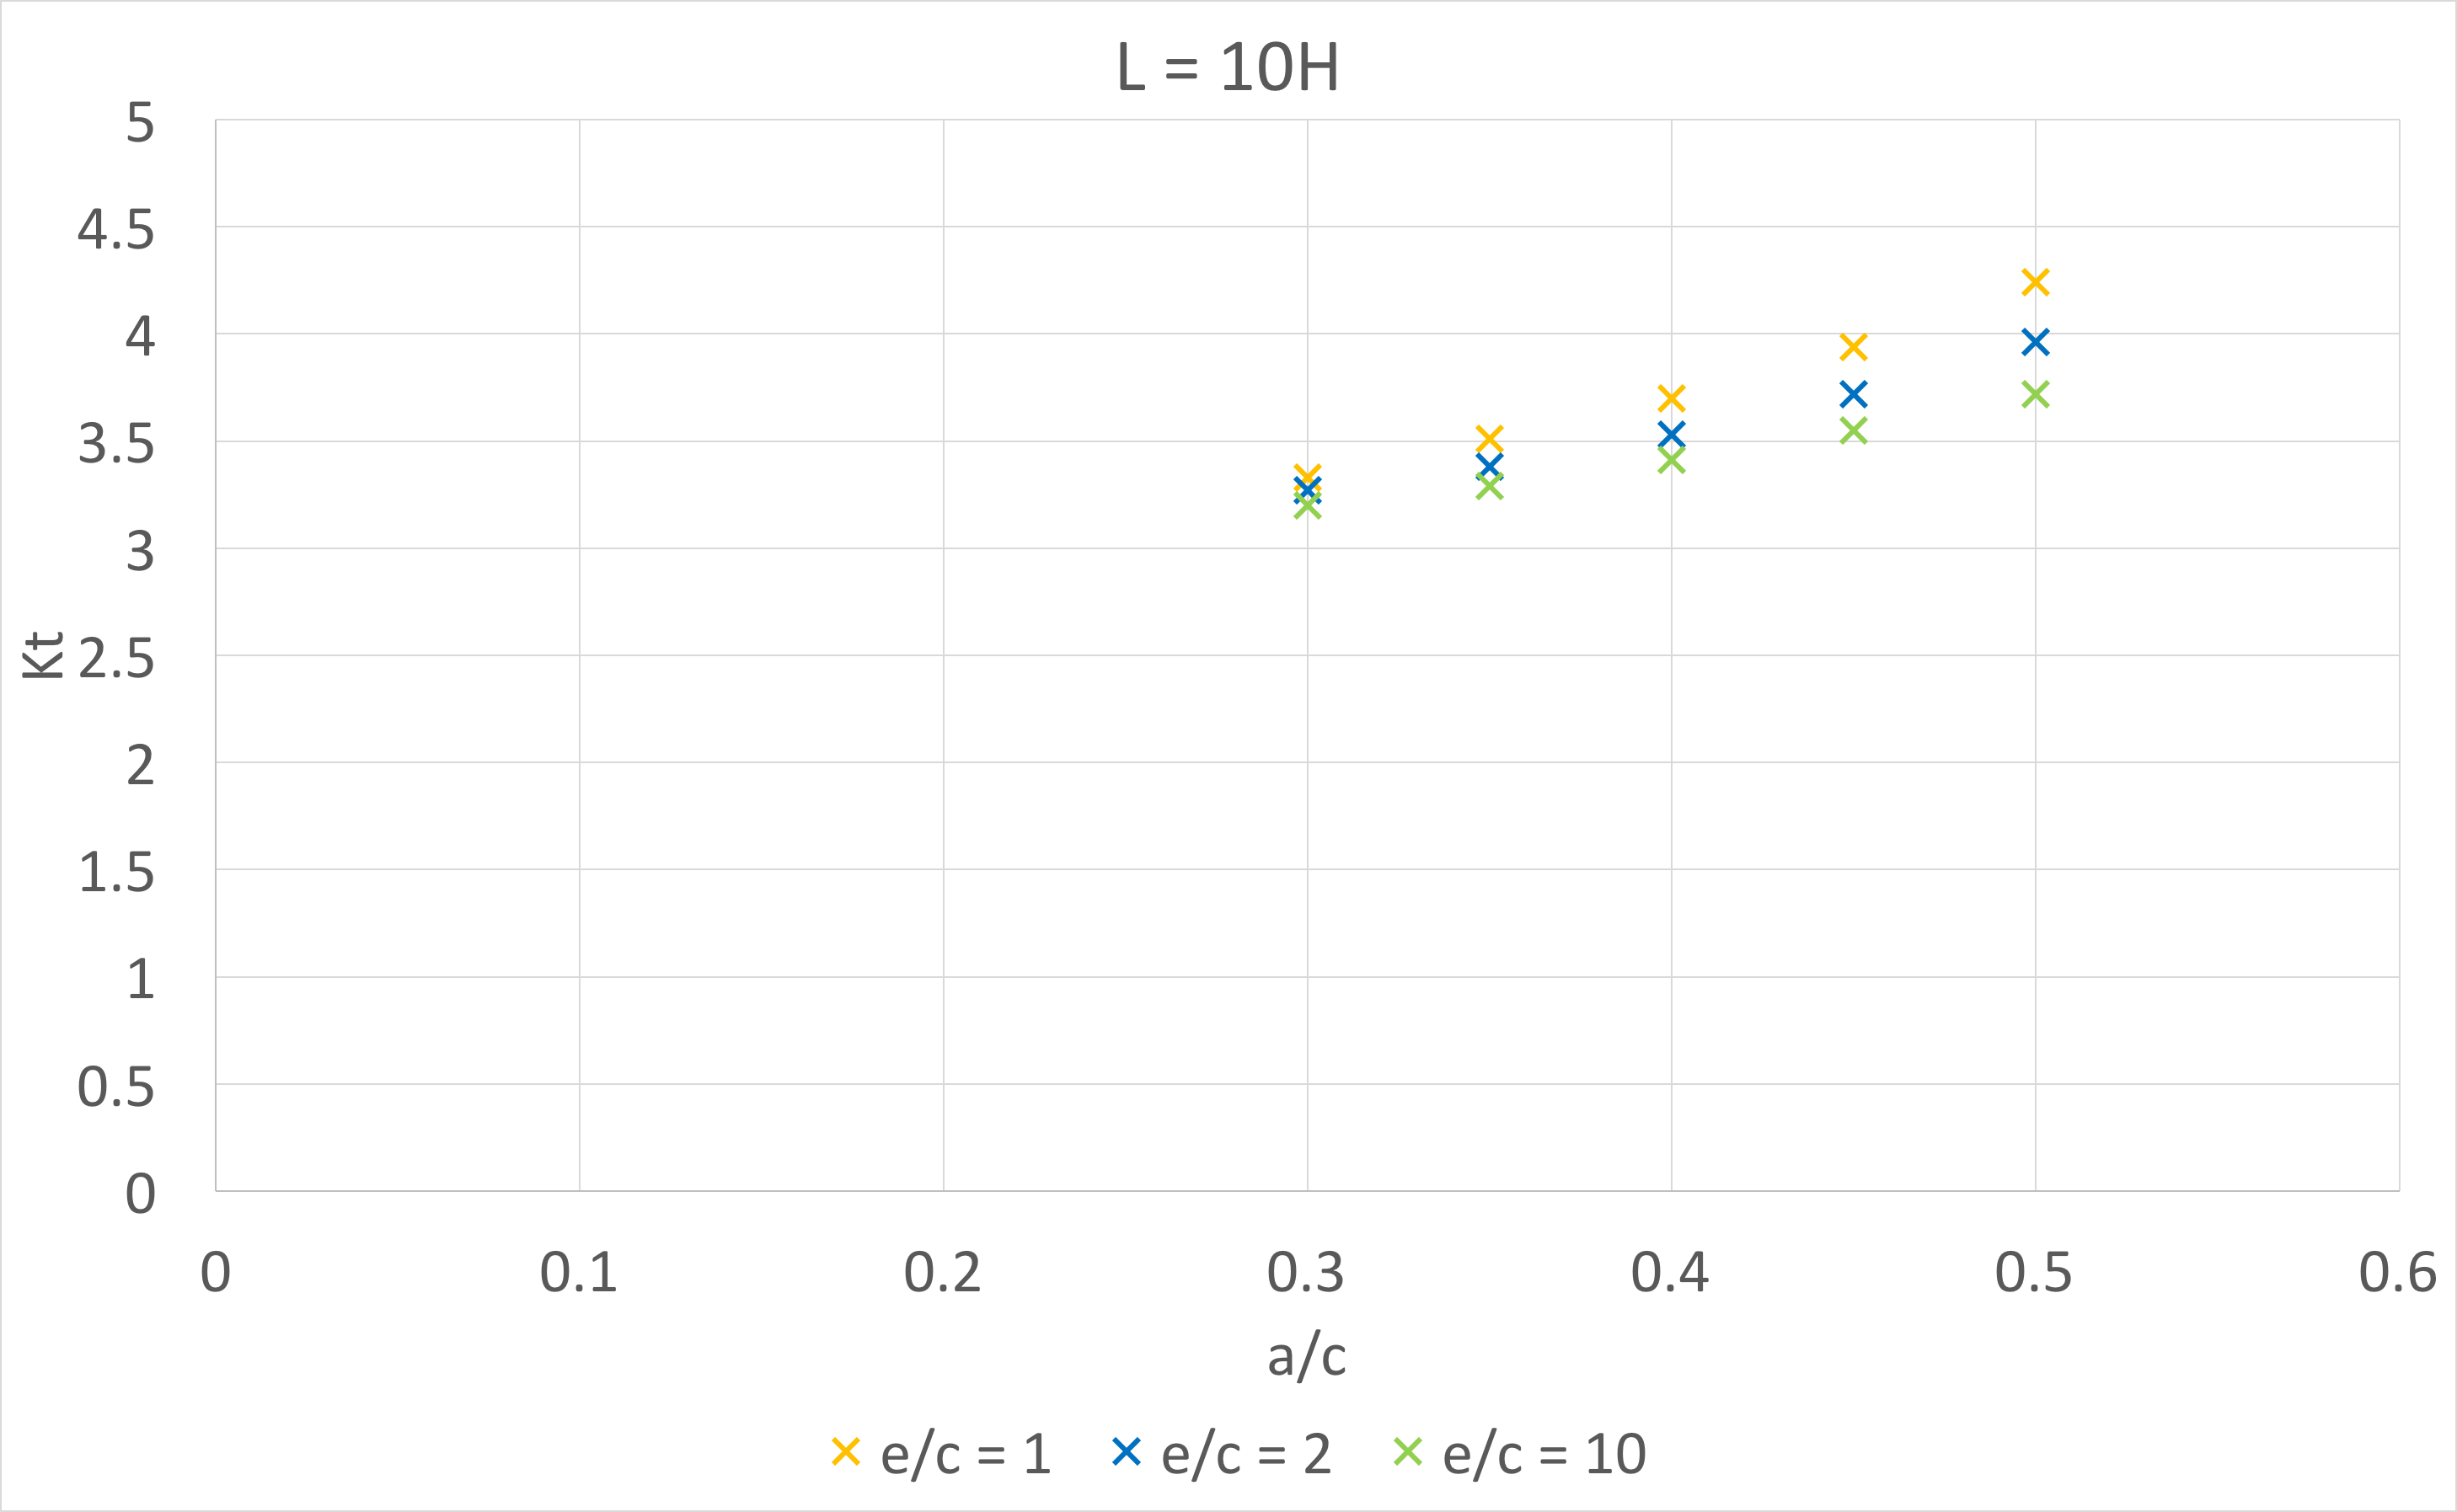
\includegraphics[height=5cm,width=0.5\textwidth]{L10.png}
    	\caption{L = 10H}
\end{figure}
\begin{figure}[!ht]
    	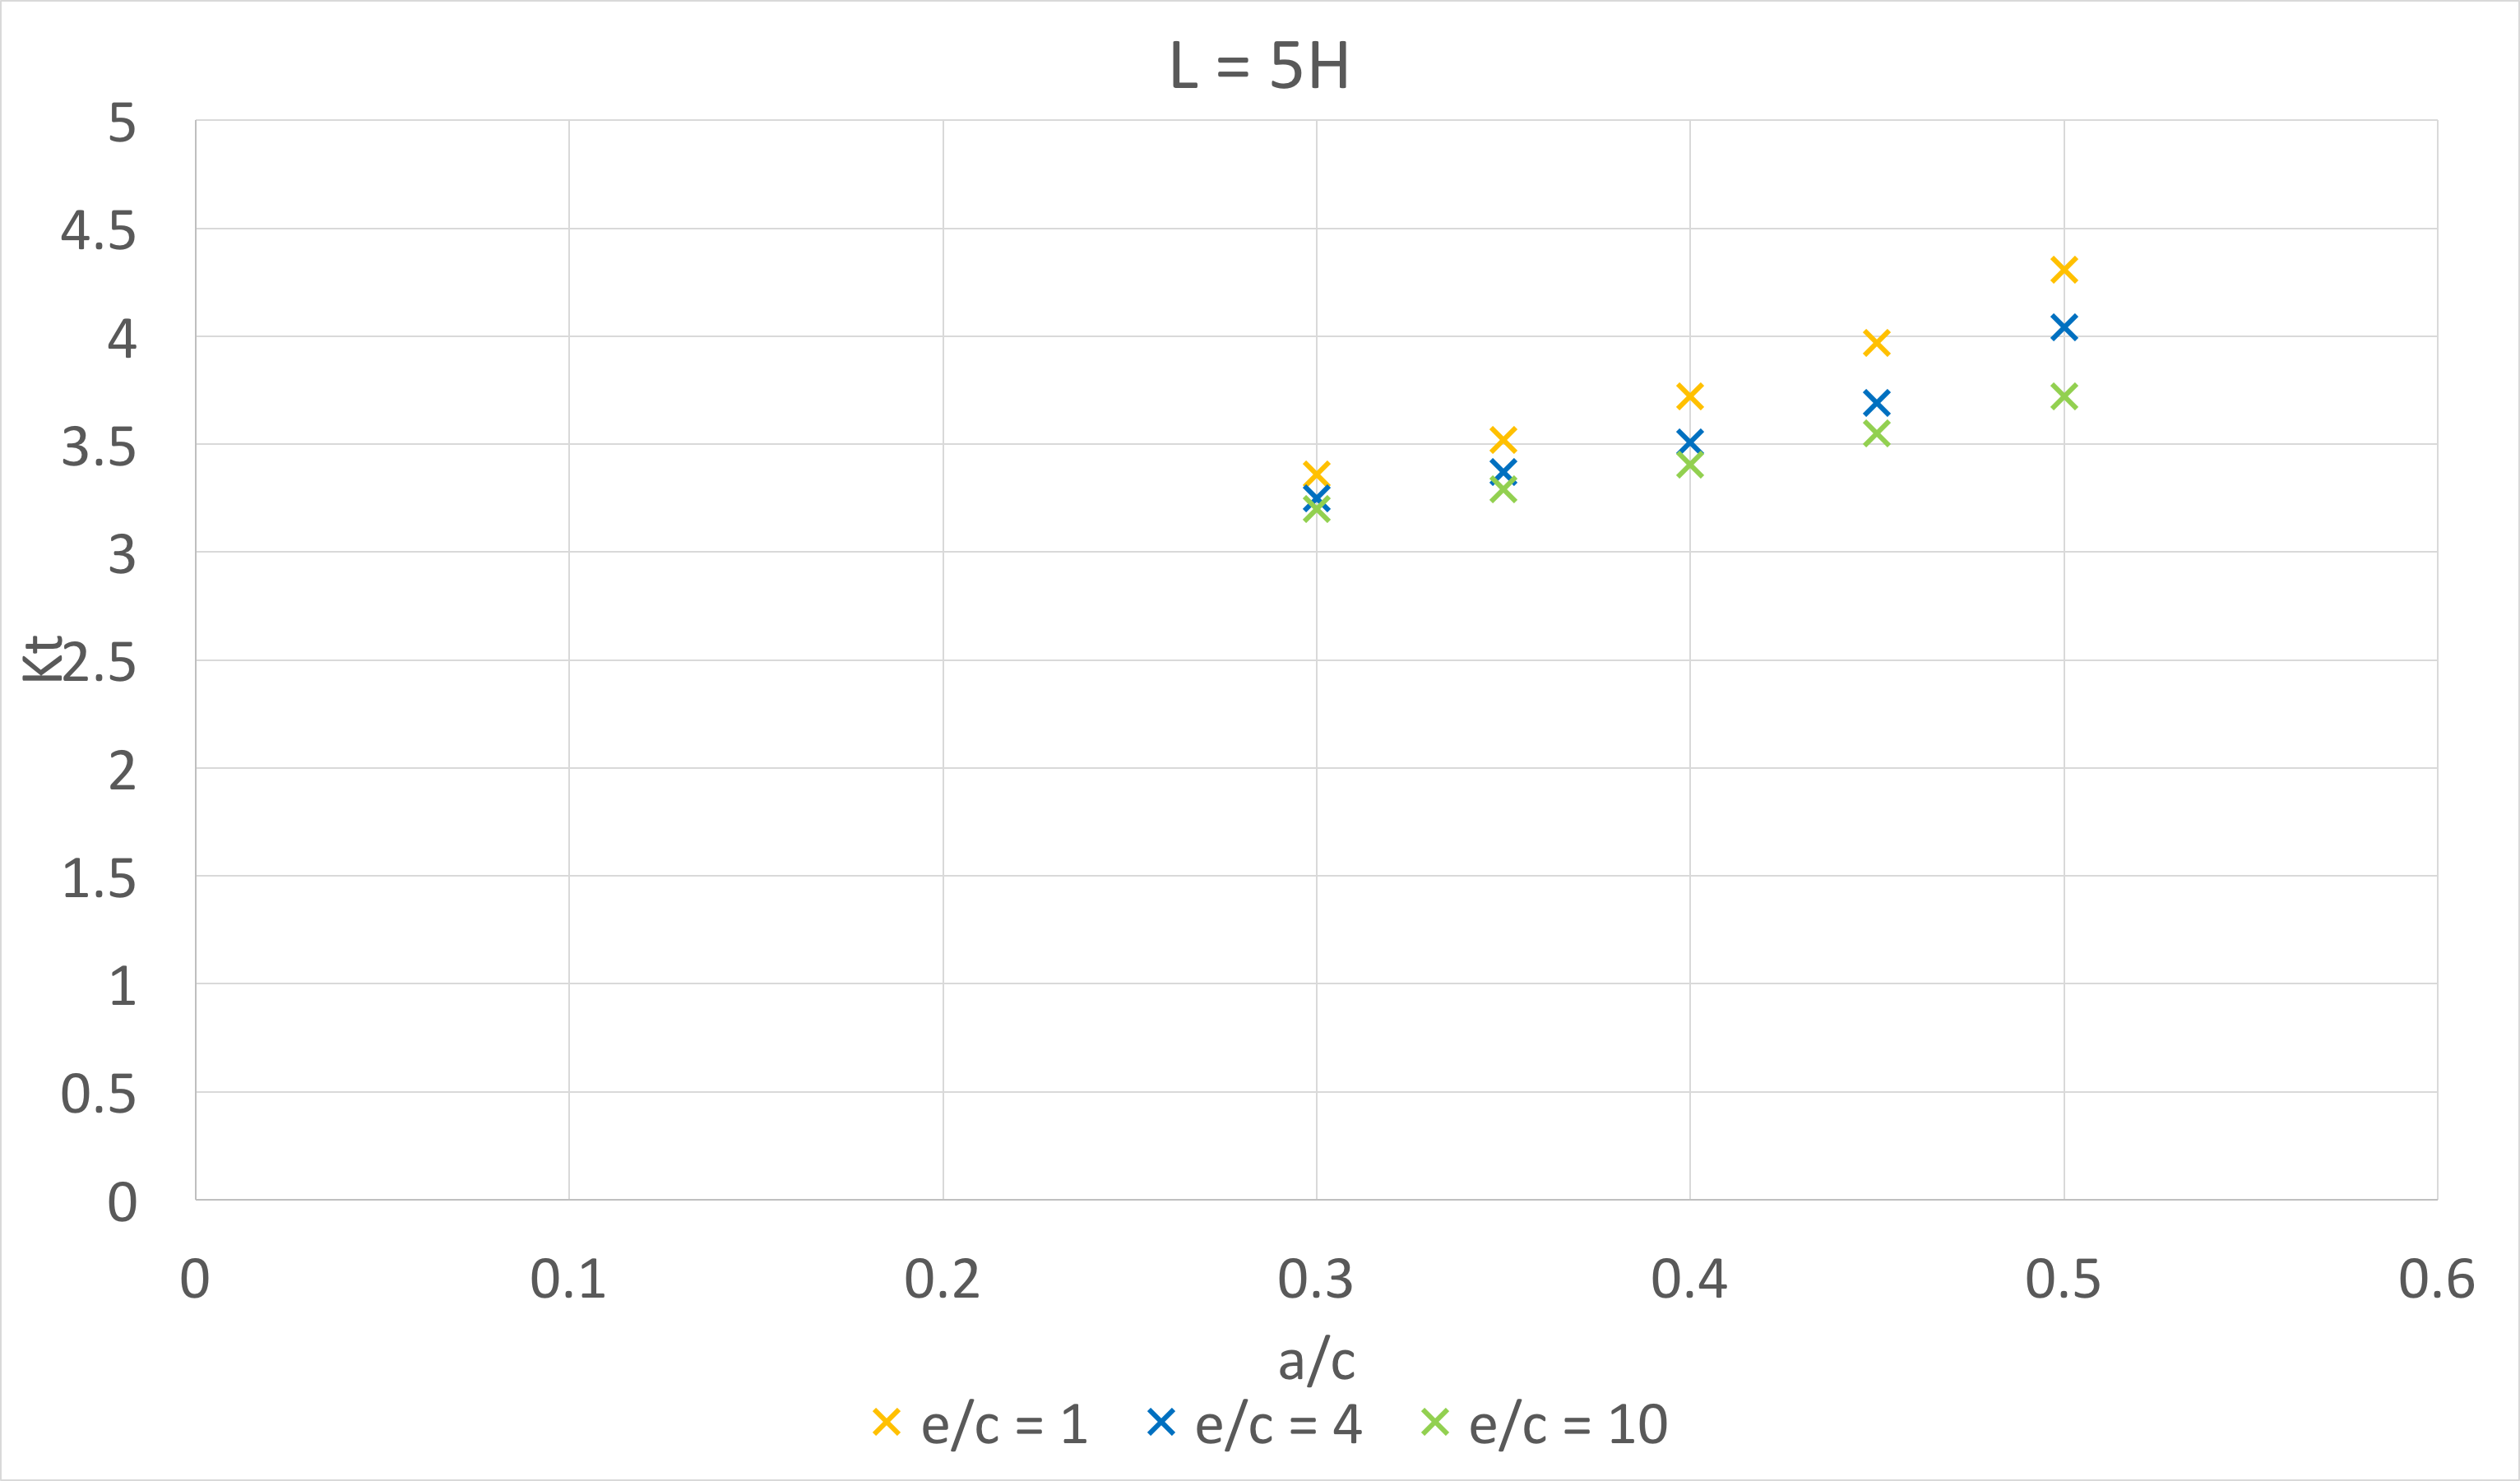
\includegraphics[height=5cm,width=0.5\textwidth]{L5.png}
    	\caption{L = 5H}
\end{figure}
\linebreak\linebreak
However, when the extremities of the data collected are considered, $L=10H$, and $L=H$, there is a very clear difference in the value of $K_{t}$. Upon studying \textit{Figures 13} \& \textit{14} it can be seen that the minimum values of $K_{t}$ are approximately the same as $K_{t} = 3.2$, when $L=10H$, and when $K_{t}= 3.22$, when $L=1H$. Meaning that there is only a percentage difference of $\%0.62$. Although when the maximum $K_{t}$ case is considered for these plates the values are $K_{t}=4.24$ for $L=10H$ and $K_{t}=5.00$ for $L=1H$, meaning that there is a difference in $K_{t}$ of $0.76$ which translates to a $\%15.2$ percentage difference. This provides further evidence for how when decreasing the plate to a state where it may no longer may be considered to be an infinite plate causes stress concentrations to be amplified around a feature.  
% Figure 13 & 14
\begin{figure}[!ht]
    	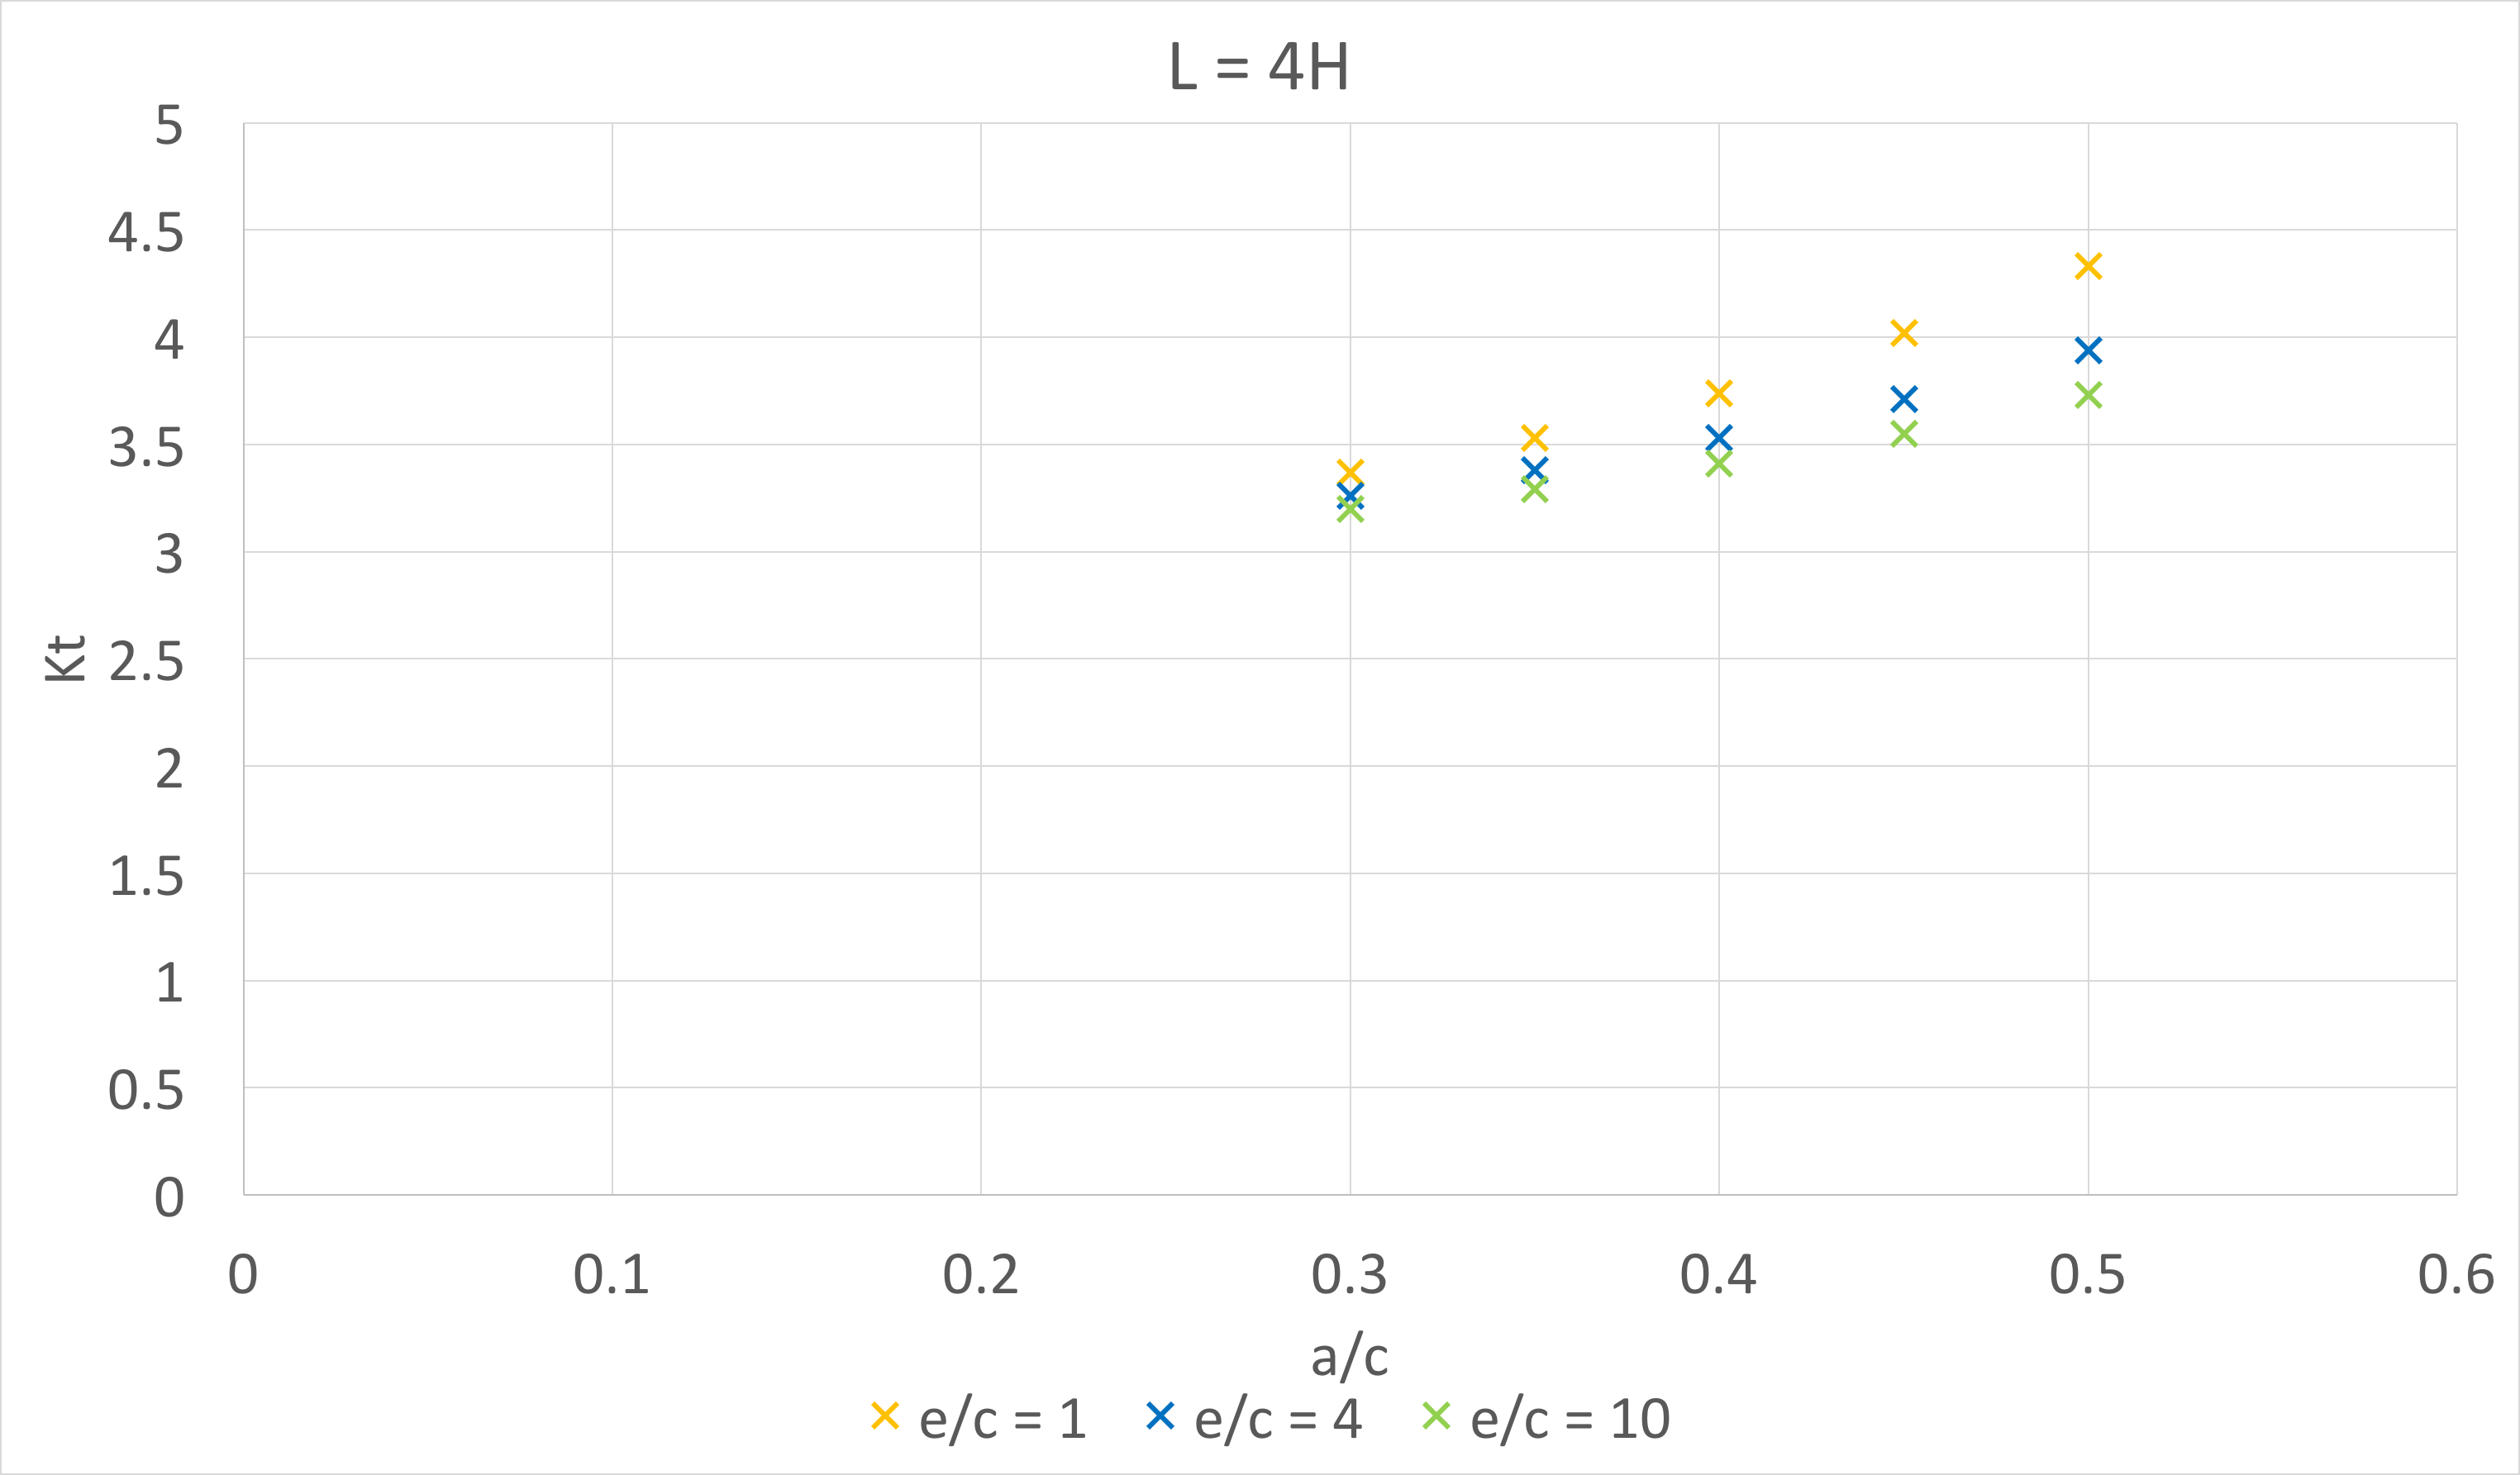
\includegraphics[width=0.5\textwidth]{L4.png}
    	\caption{L = 4H}
\end{figure}
\begin{figure}[!ht]
    	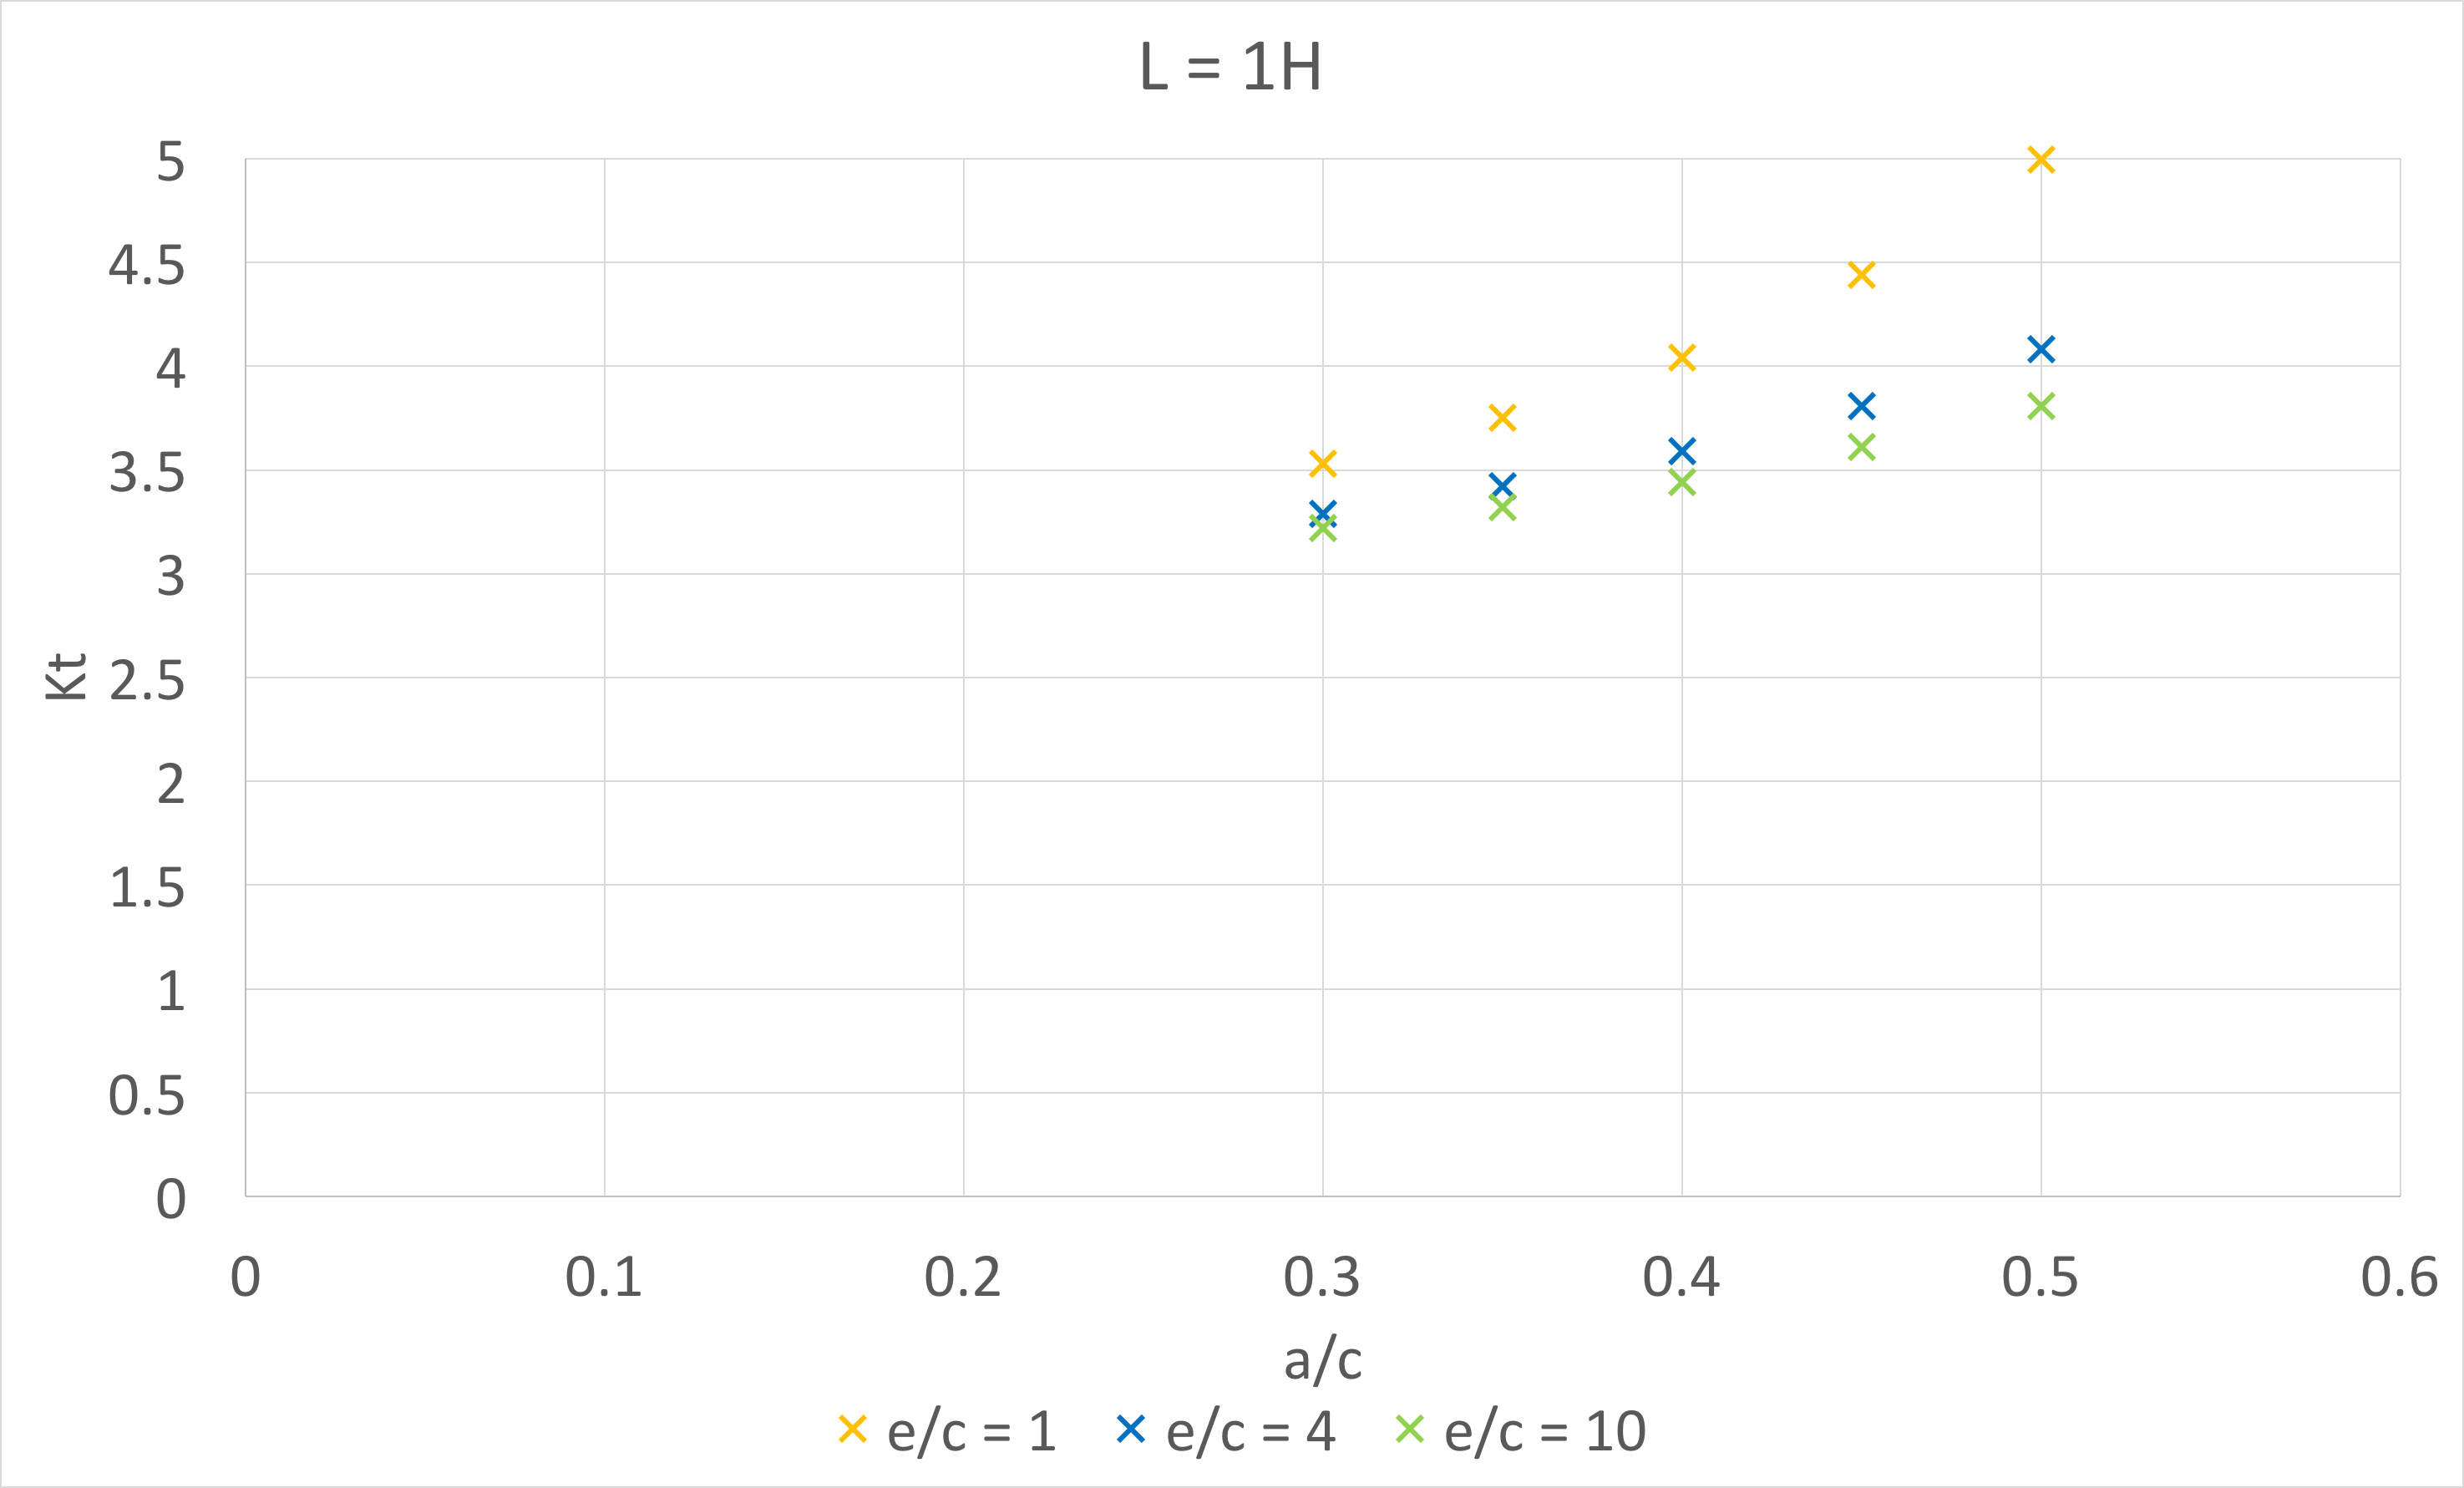
\includegraphics[width=0.5\textwidth]{L1.png}
    	\caption{L = 1H}
\end{figure}
\\ \par 
 A further observation is that when $L=10H$, which is the upper bound of the range of the plate dimensions which were considered to be infinite for which data was acquired, the smallest recorded value is $K_{t}3.2$ which does not match the value calculated in theory which states for an infinite plate $K_{t}$ should equal $3$. This implies that the assumption previously made throughout this experiment that so long as the plate has a length $\geq 5$ times its width it may be considered infinite is incorrect. Instead the value of $L$ must be greater than tested for throughout this experiment. If further experiments were to be conducted, this could be investigated by performing computational simulations at greater values of length than in this experiment, to show which value of L is required to produce $K_{t} = 3$.
%--------------------------------------------------------------------------------------------------------------------------------------------------------------------------------------------------------------------------
% CONCLUSION
%--------------------------------------------------------------------------------------------------------------------------------------------------------------------------------------------------------------------------
\section{Conclusion}
It has been verified through this experiment that introducing a circular cutout into an infinite plate will lead to a stress concentration forming around the cutout. In theory it was determined that $K_{t}$ would equal $3.0$, however the data obtained from the computational simulation showed that for a plate of length $L = 10H$ the stress concentration factor, $K_{t} = 3.2$ not the $3.0$ which the theory states should be present in an infinite plate. In addition to this it was shown that if a concentration is introduced into a plate which is not infinite it will be larger than that of an equivalent cutout in an infinite plate, and that increasing the value of$e/c$ will lead to an increase in $K_{t}$ and increasing $a/c$ will lead to an increase in $K_{t}$. Furthermore, it was shown that  the value of Poisson's ratio for the aluminium plate was, $\nu = 0.32$, which is in agreement with the stated value for an aluminium alloy.
\clearpage
%--------------------------------------------------------------------------------------------------------------------------------------------------------------------------------------------------------------------------
% REFERENCES
%--------------------------------------------------------------------------------------------------------------------------------------------------------------------------------------------------------------------------
\onecolumn
\begin{thebibliography} {9} % Begin bibliography.
\bibitem{Titanium}
AZO materials (2014, May, 27) \textit{Comparison of Titanium and Steel/Aluminium} [Online] Available: http://www.azom.com/article.aspx?ArticleID=11005

\bibitem{aeroplane}
Industry talks (2012, Dec, 12) \textit{Industrial Talks Why Titanium Is Used in the Aircraft Industry} [Online] Available: https://industrialtalks.wordpress.com/2012/12/12/why-titanium-is-used-in-the-aircraft-industry/

\bibitem{SOD}
Mattheck C and Burkhardt S (1990). \textit{A new method of structural shape optimisation based on biological growth. International Journal of Fatigue}, Vol. 12

\bibitem{LargeSystems}
G. I. N. Rozvany (1993, Oct, 4) \textit{Optimization of Large Structural Systems(Series E - Vol 231)} pp. 264

\bibitem{plates}
University of Colorado, \textit{Kirchhoff Plates Filed Equations}. [Online] Available: http://www.colorado.edu/engineering/CAS/courses.d/AFEM.d/AFEM.Ch20.d/AFEM.Ch20.pdf 

\bibitem{Kirch}
Greg Todd. \textit{Fracture Mechanics - Stress Concentrations at Holes} [Online] Available: http://www.fracturemechanics.org/hole.html

\bibitem{planestress}
UCSB College of Engineering, \textit{Plane Stress and Plane Strain} [Online] Available: https://engineering.ucsb.edu/~hpscicom/projects/stress/introge.pdf

\bibitem{Aluminium}
Engineers edge, \textit{Poisson's Ratio Metals Materials Chart} [Online] Available: http://www.engineersedge.com/materials/poissons\_ratio\_metals\_materials\_chart\_13160.htm

\textbf{Figure 1} - \textit{Fracture mechanics - Stress concentrations at Holes} Available: http://www.fracturemechanics.org/hole.html

\textbf{Figure 2} - \textit{Durham University,
School of Engineering and Computing Sciences, Level 2 Laboratory Experiment, M23 Stress Concentrations Lab Script} 

\textbf{Figure 4} -  \textit{Durham University, School of Engineering and Computing Sciences, Level 2, Module ENGI2221 : Mechanics Coursework: Stress concentrations}

\end{thebibliography} 

%-------------------------------------------------------------------------------------------------------------------------------------------------------------------------------------------------------------------------
% END REPORT 
%-------------------------------------------------------------------------------------------------------------------------------------------------------------------------------------------------------------------------
\end{document}